%%%%%%%%%%%%%%%%%%%%%%%%%%%%%%%%%%%%%
%% Master Thesis - Computer Engineering
%% Copyright 2009 Ricardo Alexandre Fiorelli, Erick Poletto
%% This document is distributed by the terms of the license
%% included in the file LICENSE.
%%%%%%%%%%%%%%%%%%%%%%%%%%%%%%%%%%%%%

\documentclass[dvips,ruledheader]{abnt}
% Foi retirado para que o texto fique em inglês
\usepackage[brazil]{babel}
%\usepackage[english]{babel}
\usepackage[latin1]{inputenc}
\usepackage[dvips]{graphicx}
\usepackage{abnt-alf}
\usepackage{latexsym}
\usepackage{psfrag}
\usepackage[center, small, bf]{caption}
\usepackage{amsmath}

% User definined packages
\usepackage{graphicx}
\usepackage{url}
\usepackage{amssymb}
\usepackage{eurofont}
\usepackage{subfig}
\usepackage{tabularx}
\usepackage{rotating}

\setcounter{tocdepth}{2} %To set the depth for numbering for the Table of Contents

% Use defined commands
\newcommand{\tn}{\tabularnewline}
\newcommand{\tnhl}{\tabularnewline\hline}
\newcommand{\hl}{\hline}

\begin{document}

\DeclareGraphicsRule{.eps.gz}{eps}{.eps.bb}{`gunzip -c #1}

%\include{capa}
%%%%%%%%%%%%%%%%%%%%%%%%%%%%%%%%%%%%%
%% Master Thesis - Computer Engineering
%% Copyright 2009 Ricardo Alexandre Fiorelli, Erick Poletto
%% This document is distributed by the terms of the license
%% included in the file LICENCE.
%%%%%%%%%%%%%%%%%%%%%%%%%%%%%%%%%%%%%

%%%%%%%%%%%%%%%%%%%%%%%%%%%%%%%%%%%%%
%% Coverpage
%%%%%%%%%%%%%%%%%%%%%%%%%%%%%%%%%%%%%

% Usando o comando \capa

\titulo{Title of the Thesis}% TODO

\autor{Erick Poletto \\ Ricardo Alexandre Fiorelli}

\orientador[Orientator:]{Prof. Chiara Francalanci}
% ou \orientador[Orientadora:\\]{Minha orientadora}

%\coorientador{Meu co-orientador}
% ou \coorientador[Co-orientadora:\\]{Minha co-orientadora}

\comentario{comments}% TODO


\instituicao{Master Thesis in Computer Engineering \par 
	Dipartimento di Elettronica ed Informazione (DEI)\par 
	Politecnico di Milano}

\local{Milan -- IT}

\data{July/2009}

\capa


% ou...
% fazendo a mao
%
% \begin{titlepage}
%
%   ... codigo da folha de rosto
%  
% \end{titlepage}


%%%%%%%%%%%%%%%%%%%%%%%%%%%%%%%%%%%%%%
%% Master Thesis - Computer Engineering
%% Copyright 2009 Ricardo Alexandre Fiorelli, Erick Poletto
%% This document is distributed by the terms of the license
%% included in the file LICENCE.
%%%%%%%%%%%%%%%%%%%%%%%%%%%%%%%%%%%%%

%%%%%%%%%%%%%%%%%%%%%%%%%%%%%%%%%%%%%
%% Folha de rosto
%%%%%%%%%%%%%%%%%%%%%%%%%%%%%%%%%%%%%

% Usando o comando \folhaderosto

\titulo{Title of the Thesis}% TODO

\autor{Erick Poletto \\ Ricardo Alexandre Fiorelli}

\begin{center}
Copyright 2009 Ricardo Alexandre Fiorelli, Erick Poletto.\\ This document is distributed by the terms of the license included in the file LICENCE.
\end{center}

\orientador[Orientator:]{Prof. Chiara Francalanci}
\coorientador[Co-orientator:]{Prof. Paolo Giacomazzo}
% ou \orientador[Orientadora:\\]{Minha orientadora}

%\coorientador{Meu co-orientador}
% ou \coorientador[Co-orientadora:\\]{Minha co-orientadora}

\comentario{}% TODO


\instituicao{Master Thesis in Computer Engineering \par 
	Dipartimento di Elettronica ed Informazione (DEI)\par 
	Politecnico di Milano}

\local{Milan -- IT}

\data{July/2009}

\folhaderosto


% ou...
% fazendo a mao
%
% \begin{titlepage}
%
%   ... codigo da folha de rosto
%  
% \end{titlepage}

%%%%%%%%%%%%%%%%%%%%%%%%%%%%%%%%%%%%%
%% Master Thesis - Computer Engineering
%% Copyright 2009 Ricardo Alexandre Fiorelli, Erick Poletto
%% This document is distributed by the terms of the license
%% included in the file LICENCE.
%%%%%%%%%%%%%%%%%%%%%%%%%%%%%%%%%%%%%

%%%%%%%%%%%%%%%%%%%%%%%%%%%%%%%%%%%%%
%% Folha de rosto
%%%%%%%%%%%%%%%%%%%%%%%%%%%%%%%%%%%%%

% Usando o comando \folhaderosto

\titulo{Title of the Thesis}% TODO

\autor{Erick Poletto \\ Ricardo Alexandre Fiorelli}

\begin{center}
Copyright 2009 Ricardo Alexandre Fiorelli, Erick Poletto.\\ This document is distributed by the terms of the license included in the file LICENCE.
\end{center}

\orientador[Orientator:]{Prof. Chiara Francalanci}
\coorientador[Co-orientator:]{Prof. Paolo Giacomazzo}
% ou \orientador[Orientadora:\\]{Minha orientadora}

%\coorientador{Meu co-orientador}
% ou \coorientador[Co-orientadora:\\]{Minha co-orientadora}

\comentario{}% TODO


\instituicao{Master Thesis in Computer Engineering \par 
	Dipartimento di Elettronica ed Informazione (DEI)\par 
	Politecnico di Milano}

\local{Milan -- IT}

\data{July/2009}

\folhaderosto


% ou...
% fazendo a mao
%
% \begin{titlepage}
%
%   ... codigo da folha de rosto
%  
% \end{titlepage}


%%%%%%%%%%%%%%%%%%%%%%%%%%%%%%%%%%%%%%
%% Master Thesis - Computer Engineering
%% Copyright 2009 Ricardo Alexandre Fiorelli, Erick Poletto
%% This document is distributed by the terms of the license
%% included in the file LICENCE.
%%%%%%%%%%%%%%%%%%%%%%%%%%%%%%%%%%%%%

%%%%%%%%%%%%%%%%%%%%%%%%%%%%%%%%%%%%%
%% 
%%%%%%%%%%%%%%%%%%%%%%%%%%%%%%%%%%%%%

\begin{folhadeaprovacao}
%Disserta��o de Mestrado sob o t�tulo \textit{``Avalia��o da qualidade da gasolina atrav�s de medidas el�tricas''}, defendida por Dehon Charles Regis %Nogueira e aprovada em 17 de janeiro de 2003, em Fortaleza, Cear�, pela banca examinadora constitu�da pelos doutores:

% TODO

\setlength{\ABNTsignthickness}{0.4pt}
\setlength{\ABNTsignwidth}{10cm}
\setlength{\ABNTsignskip}{3.5cm}

\assinatura{}% TODO

\assinatura{}% TODO

\assinatura{}% TODO

\end{folhadeaprovacao}


%%%%%%%%%%%%%%%%%%%%%%%%%%%%%%%%%%%%%%
%% Master Thesis - Computer Engineering
%% Copyright 2009 Ricardo Alexandre Fiorelli, Erick Poletto
%% This document is distributed by the terms of the license
%% included in the file LICENCE.
%%%%%%%%%%%%%%%%%%%%%%%%%%%%%%%%%%%%%

%%%%%%%%%%%%%%%%%%%%%%%%%%%%%%%%%%%%%
%% Dedicatoria
%%%%%%%%%%%%%%%%%%%%%%%%%%%%%%%%%%%%%

\ 

\vfill

\begin{flushright}
\hfill \textit{\ldots}% TODO
\end{flushright}

\vspace*{1cm}

\clearpage

%%%%%%%%%%%%%%%%%%%%%%%%%%%%%%%%%%%%%
%% Master Thesis - Computer Engineering
%% Copyright 2009 Ricardo Alexandre Fiorelli, Erick Poletto
%% This document is distributed by the terms of the license
%% included in the file LICENCE.
%%%%%%%%%%%%%%%%%%%%%%%%%%%%%%%%%%%%%

%%%%%%%%%%%%%%%%%%%%%%%%%%%%%%%%%%%%%
%% Dedicatoria
%%%%%%%%%%%%%%%%%%%%%%%%%%%%%%%%%%%%%

\ 

\vfill

\begin{flushright}
\hfill \textit{\ldots}% TODO
\end{flushright}

\vspace*{1cm}

\clearpage


%%%%%%%%%%%%%%%%%%%%%%%%%%%%%%%%%%%%%%
%% Master Thesis - Computer Engineering
%% Copyright 2009 Ricardo Alexandre Fiorelli, Erick Poletto
%% This document is distributed by the terms of the license
%% included in the file LICENCE.
%%%%%%%%%%%%%%%%%%%%%%%%%%%%%%%%%%%%%

%%%%%%%%%%%%%%%%%%%%%%%%%%%%%%%%%%%%%
%% Acknowledgements
%%%%%%%%%%%%%%%%%%%%%%%%%%%%%%%%%%%%%

\chapter*{Acknowledgements}


% Agradecimentos - � so para as pessoas que contribuiram relevantemente
% para a elabora��o do trabalho

% To our friends: Pedro Kayatt, Jobson Wadi, Rafael Sbampato, Rodrigo Roriz, Xenia Itikawa, Sarp Erdag who lended their computers in order to make possible the field benchmarks and power measurements.

% -- To professor Chiara Francalanci, blah blah blah
% TODO



%%%%%%%%%%%%%%%%%%%%%%%%%%%%%%%%%%%%%
%% Master Thesis - Computer Engineering
%% Copyright 2009 Ricardo Alexandre Fiorelli, Erick Poletto
%% This document is distributed by the terms of the license
%% included in the file LICENCE.
%%%%%%%%%%%%%%%%%%%%%%%%%%%%%%%%%%%%%

%%%%%%%%%%%%%%%%%%%%%%%%%%%%%%%%%%%%%
%% Acknowledgements
%%%%%%%%%%%%%%%%%%%%%%%%%%%%%%%%%%%%%

\chapter*{Acknowledgements}


% Agradecimentos - � so para as pessoas que contribuiram relevantemente
% para a elabora��o do trabalho

% To our friends: Pedro Kayatt, Jobson Wadi, Rafael Sbampato, Rodrigo Roriz, Xenia Itikawa, Sarp Erdag who lended their computers in order to make possible the field benchmarks and power measurements.

% -- To professor Chiara Francalanci, blah blah blah
% TODO




%%%%%%%%%%%%%%%%%%%%%%%%%%%%%%%%%%%%%%
%% Master Thesis - Computer Engineering
%% Copyright 2009 Ricardo Alexandre Fiorelli, Erick Poletto
%% This document is distributed by the terms of the license
%% included in the file LICENCE.
%%%%%%%%%%%%%%%%%%%%%%%%%%%%%%%%%%%%%

%%%%%%%%%%%%%%%%%%%%%%%%%%%%%%%%%%%%%
%% Epigrafe
%%%%%%%%%%%%%%%%%%%%%%%%%%%%%%%%%%%%%


%  Ep�grafe - � uma cita��o pertinente ao seu trabalho
%  ou que represente o seu modo de pensar. 
%  Resumindo, coloque uma frase que o(a) agrade.


\pretextualchapter{}

\vspace{17.5cm}
\begin{flushright}

\textit{``A atividade da engenharia, enquanto permanecer atividade, \\
	 pode levar a criatividade do homem a seu grau m�ximo; \\
	 mas, assim que o construtor p�ra de construir e se entrincheira \\
	 nas coisas que fez, as energias criativas se congelam, \\
	 e o pal�cio se transforma em tumba.'' \\ 
	\bfseries Marshall Berman}

\end{flushright}



%%%%%%%%%%%%%%%%%%%%%%%%%%%%%%%%%%%%%
%% Master Thesis - Computer Engineering
%% Copyright 2009 Ricardo Alexandre Fiorelli, Erick Poletto
%% This document is distributed by the terms of the license
%% included in the file LICENCE.
%%%%%%%%%%%%%%%%%%%%%%%%%%%%%%%%%%%%%

%%%%%%%%%%%%%%%%%%%%%%%%%%%%%%%%%%%%%
%% Epigrafe
%%%%%%%%%%%%%%%%%%%%%%%%%%%%%%%%%%%%%


%  Ep�grafe - � uma cita��o pertinente ao seu trabalho
%  ou que represente o seu modo de pensar. 
%  Resumindo, coloque uma frase que o(a) agrade.


\pretextualchapter{}

\vspace{17.5cm}
\begin{flushright}

\textit{``A atividade da engenharia, enquanto permanecer atividade, \\
	 pode levar a criatividade do homem a seu grau m�ximo; \\
	 mas, assim que o construtor p�ra de construir e se entrincheira \\
	 nas coisas que fez, as energias criativas se congelam, \\
	 e o pal�cio se transforma em tumba.'' \\ 
	\bfseries Marshall Berman}

\end{flushright}




%%%%%%%%%%%%%%%%%%%%%%%%%%%%%%%%%%%%%
%% Master Thesis - Computer Engineering
%% Copyright 2009 Ricardo Alexandre Fiorelli, Erick Poletto
%% This document is distributed by the terms of the license
%% included in the file LICENCE.
%%%%%%%%%%%%%%%%%%%%%%%%%%%%%%%%%%%%%

%%%%%%%%%%%%%%%%%%%%%%%%%%%%%%%%%%%%%
%% tirar esse arquivo
%% Questions and Doubts
%%%%%%%%%%%%%%%%%%%%%%%%%%%%%%%%%%%%%

\chapter*{Questions and Doubts}
    In order not to have any text not related to the thesis in the middle of the text and maybe, in the final version nobody sees it, I created this file, like that, we can put some information here and delete it in the last version. Of course, these are not the only issues related to the thesis, but it is better to have a centralized way to do that.

    The questions are:
\begin{description}
	\item[Section~\ref{sec3:components_database} or Appendix~\ref{app:sandra_benchmark_table_schema}] Do we need to insert all tables here, in appendix, or where do we need to insert the tables? Or just the database schema? These tables were taken from the SANDRA Access file.
	\item[Section~\ref{sec3:measures}] special attention to the schema of the database with measures with the measurement tool provided.
	\item[Figure~\ref{fig:power_consumption_harddrive}] Can we insert a picture with the Toms hardware logo, or do we need to port it and provide the source?
	\item[Figure~\ref{fig:installed_base_virtualized_servers}] same as above.
	\item[]
\end{description}

\begin{table}[htbp]
\centering
\begin{tabularx}{\textwidth}{|>{\bfseries}l|>{\centering}X|>{\centering}X|>{\centering}X|>{\centering}X|}
\hline
\bf{Computer Model} & \bf{\emph{Idle} with monitor on (W)} & \bf{\emph{Idle} with monitor off (W)} & \bf{Estimated Monitor Power (W)} & \bf{Processor fully stressed} \tnhl
HPdv3500el & 28.57 & 25.19 & 3.38 & 35.64 \tnhl
HPdv6580el & 62.18 & 57.14 & 5.04 & 85.27 \tnhl
Compaq-nx9420 & 78.89 & 74.65 & 4.24 & 79.64 \tnhl
Acer Aspire 6935g & 38.67 & 33.76 & 4.91 & 55.39 \tnhl
Acer Aspire 4720z & 44.57 & 39.88 & 4.69 & 67.28 \tnhl
Acer Aspire 5930G & 44.48 & 39.56 & 4.92 & 62.83 \tnhl
HP dv6000 & 43.65 & 39.12 & 4.53 & 58.95 \tnhl
Toshiba & 54.80 & 46.03 & 8.77 & 65.73 \tnhl
Fujistu AMILO Pa2548 & 60.28 & 55.40 & 4.88 & 87.40 \tnhl
Samsung Q310 & 33.60 & 26.60 & 7.00 & 48.55 \tnhl
Acer Aspire 5930G & 39.33 & 32.52 & 6.81 & 62.40 \tnhl
HP Pavilion dv6000 & 34.06 & 29.38 & 4.68 & 48.20 \tnhl
Sony Vaio SZ650N & 52.44 & 45.67 & 6.77 & 81.65 \tnhl
HP Pavilion ze2000 & 37.48 & 31.48 & 6.00 & 58.34 \tnhl
Sony Vaio v6nfw11e & 34.84 & 29.57 & 5.27 & 44.14 \tnhl
Asus F3 Series & 47.63 & 38.98 & 8.65 & 50.33 \tnhl
HP 550 & 41.31 & 33.60 & 7.71 & 48.11 \tnhl
\end{tabularx}
\caption{Measures made with the Energy Measurement Device}
\label{tab:measures}
\end{table}


\begin{table}[htbp]
\centering
\begin{tabularx}{\textwidth}{|>{\bfseries}l|>{\centering}X|>{\centering}X|>{\centering}X|>{\centering}X|}
\hline
\bf{Computer Model} & \bf{Processor Benchmark (W)} & \bf{Cache \& Memory Benchmark$^a$ (W)} & \bf{Physical Disks Benchmark (W)} \tnhl
HPdv3500el & 19.69 & 26.69 & N/A \tnhl
HPdv6580el & 32.01 & 40.06 & 2.00 \tnhl
Compaq-nx9420 & 26.93 & 36.16 & N/A \tnhl
Acer Aspire 6935g & 28.03 & 35.03 & N/A \tnhl
Acer Aspire 4720z & 19.78 & 34.57 & N/A \tnhl
Acer Aspire 5930G & 25.13 & 32.13 & N/A \tnhl
HP dv6000 & 25.00 & 34.23 & N/A \tnhl
Toshiba & 22.50 & 31.24 & N/A \tnhl
Fujistu AMILO Pa2548 & N/A & N/A & N/A \tnhl
Samsung Q310 & 26.28 & 33.28 & N/A \tnhl
Acer Aspire 5930G & 38.60 & 47.63 & N/A \tnhl
HP Pavilion dv6000 & 12.95 & 31.84 & N/A \tnhl
Sony Vaio SZ650N & 28.99 & 49.68 & N/A \tnhl
HP Pavilion ze2000 & 14.62 & 17.86 & N/A \tnhl
Sony Vaio v6nfw11e & 35.08 & 42.08 & N/A \tnhl
Asus F3 Series & 12.44 & 28.53 & N/A \tnhl
HP 550 & 29.63 & 44.42 & N/A \tnhl
\end{tabularx}\linebreak
$^a$ chipset + processor + memory\linebreak
$N/A$ Not Returned a Valuable Result
\caption{Measures Resulted from Benchmark with SANDRA}
\label{tab:measures_sandra}
\end{table}

\begin{table}[htbp]
\centering
\begin{tabular}{|>{\bfseries}l|l|}
\hline
\bf{Computer Model} & \bf{Processor Model} \tnhl
HPdv3500el & Intel Core Duo P8400 @ 2.26GHz \tnhl
HPdv6580el & Intel Core Duo T7300 @ 2.00GHz \tnhl
Compaq-nx9420 & Intel Core Duo T2400 @ 1.83 GHz \tnhl
Acer Aspire 6935g & Intel Core Duo T6400 @ 2.00GHz  \tnhl
Acer Aspire 4720z & Intel Core Duo T2310 @ 1.66 GHz \tnhl
Acer Aspire 5930G & Intel Core 2  P7350 @ 2.0GHz \tnhl
HP dv6000 & Intel Core Duo T5600 @ 1.83GHz \tnhl
Toshiba & Intel Core Duo T2300 @ 1.66 GHz \tnhl
Fujistu AMILO Pa2548 & AMD Turion 64 X2 TL-58 @ 1.9GHz \tnhl
Samsung Q310 & Intel Core Duo P7350 @ 2.00GHz  \tnhl
Acer Aspire 5930G & Intel Core Duo T9400 @ 2.53GHz \tnhl
HP Pavilion dv6000 & Intel Core Duo T5450 @ 1.66GHz \tnhl
Sony Vaio SZ650N & Intel Core Duo T7500 @ 2.20 GHz \tnhl
HP Pavilion ze2000 & Intel Pentium M 1.60 GHz \tnhl
Sony Vaio v6nfw11e & Intel Core Duo P8400 @ 2.26 GHz \tnhl
Asus F3 Series & Intel Core Duo T7300 @ 2.00GHz \tnhl
HP 550 & Intel Celeron 530 @ 1.73 GHz \tnhl
\end{tabular}
\caption{Processor Contained in each Measured Computer}
\label{tab:computer_processor}
\end{table}


\begin{table}[htbp]
\centering
\begin{tabularx}{0.7\textwidth}{|l|>{\centering}X|}
\hline
\bf{Processor Model} & \bf{Processor nominal power (W)} \tnhl
Intel Core Duo P8400 @ 2.26GHz & 25 \tnhl
Intel Core Duo T7300 @ 2.00GHz & 35 \tnhl
Intel Core Duo T2400 @ 1.83 GHz & 31 \tnhl
Intel Core Duo T6400 @ 2.00GHz  & 35 \tnhl
Intel Core Duo T2310 @ 1.66 GHz & 35 \tnhl
Intel Core 2  P7350 @ 2.0GHz & 25 \tnhl
Intel Core Duo T5600 @ 1.83GHz & 34 \tnhl
Intel Core Duo T2300 @ 1.66 GHz & 31 \tnhl
AMD Turion 64 X2 TL-58 @ 1.9GHz & 31 \tnhl
Intel Core Duo P7350 @ 2.00GHz  & 25 \tnhl
Intel Core Duo T9400 @ 2.53GHz & 35 \tnhl
Intel Core Duo T5450 @ 1.66GHz & 35 \tnhl
Intel Core Duo T7500 @ 2.20 GHz & 35 \tnhl
Intel Pentium M 1.60 GHz & 35 \tnhl
Intel Core Duo P8400 @ 2.26 GHz & 25 \tnhl
Intel Core Duo T7300 @ 2.00GHz & 35 \tnhl
Intel Celeron 530 @ 1.73 GHz & 27 \tnhl
\end{tabularx}
\caption{Manufacturer Specification}
\label{tab:manufacturer_specification}
\end{table}




\begin{table}[htbp]
\centering
\begin{tabularx}{\textwidth}{|>{\bfseries}l|>{\centering}X|>{\centering}X|>{\centering}X|}
\hline
\bf{Computer Model} & \bf{Benchmark Processor Power (W)} & \bf{Nominal Processor Power (W)} & \bf{Incompatible Results} \tnhl
HPdv3500el & 19.69 & 25 & \bf{} \tnhl
HPdv6580el & 32.01 & 35 & \bf{} \tnhl
Compaq-nx9420 & 26.93 & 31 & \bf{} \tnhl
Acer Aspire 6935g & 28.03 & 35 & \bf{} \tnhl
Acer Aspire 4720z & 19.78 & 35 & \bf{} \tnhl
Acer Aspire 5930G & 25.13 & 25 & \bf{x} \tnhl
HP dv6000 & 25 & 34 & \bf{} \tnhl
Toshiba & 22.5 & 31 & \bf{} \tnhl
Fujistu AMILO Pa2548 & N/A & 31 & \bf{} \tnhl
Samsung Q310 & 26.28 & 25 & \bf{x} \tnhl
Acer Aspire 5930G & 38.6 & 35 & \bf{x} \tnhl
HP Pavilion dv6000 & 12.95 & 35 & \bf{} \tnhl
Sony Vaio SZ650N & 28.99 & 35 & \bf{} \tnhl
HP Pavilion ze2000 & 14.62 & 35 & \bf{} \tnhl
Sony Vaio v6nfw11e & 35.08 & 25 & \bf{x} \tnhl
Asus F3 Series & 12.44 & 35 &  \tnhl
HP 550 & 29.63 & 27 & \bf{x} \tnhl
\end{tabularx}\linebreak
$N/A$ Not Returned a Valuable Result
\caption{Processor Specifications' Results }
\label{tab:results_spec_processor}
\end{table}



\begin{table}[htbp]
\centering
\begin{tabularx}{\textwidth}{|>{\bfseries}l|>{\centering}X|>{\centering}X|>{\centering}X|}
\hline
\bf{Computer Model} & \bf{Measurement Result: \emph{Idle} With Monitor Off (W)} & \bf{Estimated PSU Power$^a$ (W)} & \bf{Measured Power$^b$ (W)} \tnhl
HPdv3500el & 25.19 & 6.30 & 18.89 \tnhl
HPdv6580el & 57.14 & 14.29 & 42.86 \tnhl
Compaq-nx9420 & 74.65 & 18.66 & 55.99 \tnhl
Acer Aspire 6935g & 33.76 & 8.44 & 25.32 \tnhl
Acer Aspire 4720z & 39.88 & 9.97 & 29.91 \tnhl
Acer Aspire 5930G & 39.56 & 9.89 & 29.67 \tnhl
HP dv6000 & 39.12 & 9.78 & 29.34 \tnhl
Toshiba & 46.03 & 11.51 & 34.52 \tnhl
Fujistu AMILO Pa2548 & 55.40 & 13.85 & 41.55 \tnhl
Samsung Q310 & 26.60 & 6.65 & 19.95 \tnhl
Acer Aspire 5930G & 32.52 & 8.13 & 24.39 \tnhl
HP Pavilion dv6000 & 29.38 & 7.35 & 22.04 \tnhl
Sony Vaio SZ650N & 45.67 & 11.42 & 34.25 \tnhl
HP Pavilion ze2000 & 31.48 & 7.87 & 23.61 \tnhl
Sony Vaio v6nfw11e & 29.57 & 7.39 & 22.18 \tnhl
Asus F3 Series & 38.98 & 9.75 & 29.24 \tnhl
HP 550 & 33.60 & 8.40 & 25.20 \tnhl
\end{tabularx}\linebreak
$^a$ at 75\% Efficiency\linebreak
$^b$ processor/chipset/memory
\caption{Measures with Processor in \emph{idle} state}
\label{tab:measures_idle}
\end{table}




\begin{table}[htbp]
\centering
\begin{tabularx}{\textwidth}{|>{\bfseries}l|>{\centering}X|>{\centering}X|>{\centering}X|}
\hline
\bf{Computer Model} & \bf{Measurement result: \emph{Fully Stressed}$^a$ (W)} & \bf{Estimated PSU Power$^b$ (W)} & \bf{Measured power$^c$ (W)} \tnhl
HPdv3500el & 32.26 & 8.07 & 24.20 \tnhl
HPdv6580el & 80.23 & 20.06 & 60.17 \tnhl
Compaq-nx9420 & 75.40 & 18.85 & 56.55 \tnhl
Acer Aspire 6935g & 50.48 & 12.62 & 37.86 \tnhl
Acer Aspire 4720z & 62.59 & 15.65 & 46.94 \tnhl
Acer Aspire 5930G & 57.91 & 14.48 & 43.43 \tnhl
HP dv6000 & 54.42 & 13.61 & 40.82 \tnhl
Toshiba & 56.96 & 14.24 & 42.72 \tnhl
Fujistu AMILO Pa2548 & 82.52 & 20.63 & 61.89 \tnhl
Samsung Q310 & 41.55 & 10.39 & 31.16 \tnhl
Acer Aspire 5930G & 55.59 & 13.90 & 41.69 \tnhl
HP Pavilion dv6000 & 43.52 & 10.88 & 32.64 \tnhl
Sony Vaio SZ650N & 74.88 & 18.72 & 56.16 \tnhl
HP Pavilion ze2000 & 52.34 & 13.09 & 39.26 \tnhl
Sony Vaio v6nfw11e & 38.87 & 9.72 & 29.15 \tnhl
Asus F3 Series & 41.68 & 10.42 & 31.26 \tnhl
HP 550 & 40.40 & 10.10 & 30.30 \tnhl
\end{tabularx}\linebreak
$^a$ estimated monitor power
$^b$ at 75\% efficiency \linebreak
$^c$processor/chipset/memory
\caption{Measures with Processor \emph{Fully Stressed}}
\label{tab:measures_fully_stressed}
\end{table}



\begin{table}[htbp]
\centering
\begin{tabularx}{\textwidth}{|>{\bfseries}l|>{\centering}X|>{\centering}X|>{\centering}X|}
\hline
\bf{Computer Model} & \bf{Sandra Benchmark: Measurement of Consumption}$^a$ & \bf{Measured Consumption}$^a$ & \bf{Percentual delta over the measured values} \tnhl
HPdv3500el & 26.69 & 18.89 & 41\% \tnhl
HPdv6580el & 40.06 & 42.86 & 7\% \tnhl
Compaq-nx9420 & 36.16 & 55.99 & 35\% \tnhl
Acer Aspire 6935g & 35.03 & 25.32 & 38\% \tnhl
Acer Aspire 4720z & 34.57 & 29.91 & 16\% \tnhl
Acer Aspire 5930G & 32.13 & 29.67 & 8\% \tnhl
HP dv6000 & 34.23 & 29.34 & 17\% \tnhl
Toshiba & 31.24 & 34.52 & 10\% \tnhl
Samsung Q310 & 33.28 & 19.95 & 67\% \tnhl
Acer Aspire 5930G & 47.63 & 24.39 & 95\% \tnhl
HP Pavilion dv6000 & 31.84 & 22.04 & 44\% \tnhl
Sony Vaio SZ650N & 49.68 & 34.25 & 45\% \tnhl
HP Pavilion ze2000 & 17.86 & 23.61 & 24\% \tnhl
Sony Vaio v6nfw11e & 42.08 & 22.18 & 90\% \tnhl
Asus F3 Series & 28.53 & 29.24 & 2\% \tnhl
HP 550 & 44.42 & 25.20 & 76\% \tnhl
 &  & \bf{Average delta:} & \bf{39\%} \tnhl
\end{tabularx}\linebreak
$^a$ chipset+processor+memory
\caption{Results for Processor in \emph{Idle} State}
\label{tab:results_final_idle}
\end{table}



\begin{table}[htbp]
\centering
\begin{tabularx}{\textwidth}{|>{\bfseries}l|>{\centering}X|>{\centering}X|>{\centering}X|}
\hline
\bf{Computer Model} & \bf{Sandra Benchmark: measurement of Consumption}$^a$ & \bf{Measured Consumption}$^a$ & \bf{Percentual delta over the measured values} \tnhl
HPdv3500el & 26.69 & 24.20 & 10\% \tnhl
HPdv6580el & 40.06 & 60.17 & 33\% \tnhl
Compaq-nx9420 & 36.16 & 56.55 & 36\% \tnhl
Acer Aspire 6935g & 35.03 & 37.86 & 7\% \tnhl
Acer Aspire 4720z & 34.57 & 46.94 & 26\% \tnhl
Acer Aspire 5930G & 32.13 & 43.43 & 26\% \tnhl
HP dv6000 & 34.23 & 40.82 & 16\% \tnhl
Toshiba & 31.24 & 42.72 & 27\% \tnhl
Samsung Q310 & 33.28 & 31.16 & 7\% \tnhl
Acer Aspire 5930G & 47.63 & 41.69 & 14\% \tnhl
HP Pavilion dv6000 & 31.84 & 32.64 & 2\% \tnhl
Sony Vaio SZ650N & 49.68 & 56.16 & 12\% \tnhl
HP Pavilion ze2000 & 17.86 & 39.26 & 55\% \tnhl
Sony Vaio v6nfw11e & 42.08 & 29.15 & 44\% \tnhl
Asus F3 Series & 28.53 & 31.26 & 9\% \tnhl
HP 550 & 44.42 & 30.30 & 47\% \tnhl
 &  & \bf{Average delta:} & \bf{23\%} \tnhl
\end{tabularx}\linebreak
$^a$ chipset+processor+memory
\caption{Results for Processor \emph{Fully Stressed}}
\label{tab:results_final_fully_stressed}
\end{table}









 %XXX tirar essa parte na versao final da tese

%%%%%%%%%%%%%%%%%%%%%%%%%%%%%%%%%%%%%
%% Master Thesis - Computer Engineering
%% Copyright 2009 Ricardo Alexandre Fiorelli, Erick Poletto
%% This document is distributed by the terms of the license
%% included in the file LICENCE.
%%%%%%%%%%%%%%%%%%%%%%%%%%%%%%%%%%%%%

%%%%%%%%%%%%%%%%%%%%%%%%%%%%%%%%%%%%%
%% Abreviations
%%%%%%%%%%%%%%%%%%%%%%%%%%%%%%%%%%%%%

\chapter*{Glossary of Abrevitations}


% Abreviações dos termos usados no trabalho

\begin{center}
	\begin{tabular}{|l|l|} \hline
	    x       &   x                                           \tnhl
	    CIO     &   Chief Information Officer                   \tnhl
	    CPU     &   Central Processing Unit                     \tnhl
	    DDR     &   Double-Data Rate                            \tnhl
        HVAC    &                                               \tnhl
	    HDD     &   Hard-disk Drive                             \tnhl
	    ICT     &   Information and Communcation Technology     \tnhl
	    LTO     &   Linear Tape-Open                            \tnhl
		MFD     &   Multi Function Devices                      \tnhl
    	MPN     &   Manufacturer Part Number                    \tnhl
    	OS      &   Operational System                          \tnhl
    	PC      &   Personal Computer                           \tnhl
    	PDU     &                                               \tnhl
    	PSU     &   Power Supply Unit                           \tnhl
    	RAID    &                                               \tnhl
		ROI     &   Return on Investment                        \tnhl
		ROM     &   Read-Only Memory                            \tnhl
		SaaS    &   Software as a Service                       \tnhl
		SDRAM   &   Synchronous Dynamic Random Access Memory    \tnhl
		SAN     &   Storage-Area Networks                       \tnhl
		TCO     &   Total Cost of Ownership                     \tnhl
		VM      &   Virtual Machine                             \tnhl
		VPN     &   Virtual Private Network                     \tnhl
		x       &   x                                           \tnhl
	\end{tabular}
	\label{tab:glossary_of_abbreviations}
\end{center}
% TODO


%%%%%%%%%%%%%%%%%%%%%%%%%%%%%%%%%%%%%
%% Master Thesis - Computer Engineering
%% Copyright 2009 Ricardo Alexandre Fiorelli, Erick Poletto
%% This document is distributed by the terms of the license
%% included in the file LICENCE.
%%%%%%%%%%%%%%%%%%%%%%%%%%%%%%%%%%%%%

%%%%%%%%%%%%%%%%%%%%%%%%%%%%%%%%%%%%%
%% Abstract
%%%%%%%%%%%%%%%%%%%%%%%%%%%%%%%%%%%%%


\begin{abstract} 
\label{abstract}
% Apresenta��o concisa dos pontos relevantes, dando uma visao rapida e
% clara do conte�do do trabalho.
% TODO

\end{abstract}


\tableofcontents

\listoffigures
\listoftables

%\include{motivacao}
%%%%%%%%%%%%%%%%%%%%%%%%%%%%%%%%%%%%%%
%% Master Thesis - Computer Engineering
%% Copyright 2009 Ricardo Alexandre Fiorelli, Erick Poletto
%% This document is distributed by the terms of the license
%% included in the file LICENCE.
%%%%%%%%%%%%%%%%%%%%%%%%%%%%%%%%%%%%%

%%%%%%%%%%%%%%%%%%%%%%%%%%%%%%%%%%%%%
%% First Chapter
%% Motivation
%%%%%%%%%%%%%%%%%%%%%%%%%%%%%%%%%%%%%

% \chapter*{Motivation} \label{motivation}

% Mostrar o que levou a realiza��o do trabalho, e as motiva��es para que o problema seja entendido.
% Situa��o do leitor no contexto
%O greenict tem sido muito importatne para o mundo, as empresas, depois da crise economica, comecaram a ver que é importante, pois, reduz muitos custos, além de contribuirem apra o meio ambiente\ldots bla bla bla

    %TODO
    





%%%%%%%%%%%%%%%%%%%%%%%%%%%%%%%%%%%%%
%% Master Thesis - Computer Engineering
%% Copyright 2009 Ricardo Alexandre Fiorelli, Erick Poletto
%% This document is distributed by the terms of the license
%% included in the file LICENCE.
%%%%%%%%%%%%%%%%%%%%%%%%%%%%%%%%%%%%%

%%%%%%%%%%%%%%%%%%%%%%%%%%%%%%%%%%%%%
%% First Chapter
%% Introduction
%%%%%%%%%%%%%%%%%%%%%%%%%%%%%%%%%%%%%


\chapter{Introduction} \label{chap1:introduction}


%     This is a general introduction to what the thesis is all about – it is ust a description of the contents
% of each section. Briefly summarize the question (you will be stating the question in detail later),
% some of the reasons why it is a worthwhile question, and perhaps give an overview of your main
% results. This is a birds-eye view of the answers to the main questions answered in the thesis (see
% above).

\section{Motivation} \label{sec1:motivation}
% Mostrar o que levou a realiza��o do trabalho, e as motiva��es para que o problema seja entendido.
% Situa��o do leitor no contexto
%O greenict tem sido muito importatne para o mundo, as empresas, depois da crise economica, comecaram a ver que é importante, pois, reduz muitos custos, além de contribuirem apra o meio ambiente\ldots bla bla bla

% o consumo nao eh de 25% do que o planeta ainda tem. mas sim de 125% do que ele pode renovar a cada ano... esse eh o valor fixo, nao a taxa de crescimento
    The planet is threatened by global warming. The progressive pressure we impose to the environment has already exceeded the limits imposed by the available natural resources. In actual figures, it can be stated that, each year, 125\% of the renewal capacity of natural resources is currently consumed. If the growth continues at this rate, in 2050 we will be consuming more than twice the production capacity of the planet Earth~\cite{Townsend:2002:2050}. 
    
    The seek for environmental friendly solutions is spreading throughout all the economic sectors and consumers have become more aware of environmental issues and thus opt for products and services of companies which have proven to be more ecologically friendly. Moreover, it is possible to say that we will soon enter in a green trend - if we are not already in it - where environmental policies will be executed without economical or political pressure, but rather as a necessary measure for the sustainability of the business. In a following phase companies will perceive green solutions as a competitive differential instead of a necessary preoccupation thereby giving the green issue a push towards being a definitive part of the business.
        
    In the last years, the concept of Green ICT has been increasingly popular by the mantra of \emph{Going Green}. A study from Info-Tech Research Group~\cite{info-tech07}, made in U.S.A., believes that the increasing interest in adopting a green solution is beginning to generate meaningful actions. However, there exists a big gap between what companies think it is a green ICT solution and what they are really doing about it. This same study states that ``Info-Tech expects continued interest in green IT strategies and significant traction among those initiatives that both reduce waste and reduce cost. As enterprises begin to translate concern for green into practice, we expect higher spending in many leading areas such as data center design, virtualization and consolidation, print optimization, and system management tools''.
    
    The current situation is that there exists a high interest in the issue, yet scarce adoption. Nonetheless, companies have reached the consensus that it is necessary to start changing their minds towards green thoughts. So, leading industries and governments have started a proactive \emph{Going Green} promotion to expand the existent market. Measures taken in favor of this green market include the allocation of a significant amount of money in researches in the area. Besides that, it is important to notice that as soon as information related of careful management of energy consumption starts to spread, it will start to attract the companies attention. The first step will be to start to study the impact of environmental harm and power consumption in the TCO accountancies.
    
    The most important benefit of a Green ICT strategy is the reduction of costs related to the energy consumption. Some studies says that the costs with power and cooling in data centers can reach up to 20\% of the IT cost. In the economic sector, the potential savings for companies could be huge and simple actions can have big impacts in the organization. As David Frampton, VP general manager of Cisco's LAN switching business unit, explained to Reuters~\cite{Chestney2009}, ``a bank branch could save nearly \euro40,000 (US\$53,020) just by turning off phones and wireless access points outside business hours''. Following the same pattern, last year, Symantec launched a study named ``State of the Data Center Report 2008'', in which the social responsibility was the least important reason for applying a Green initiative. It states instead that \emph{reduction of costs} and \emph{reduction of power consumption} are the most important reasons to invest in such idea. 
    
    Another benefit is that Green ICT can be used as a \emph{marketing strategy} and with the growing popularity of the issue, vendors have started to put green labels on their products and consumers also started to seek for green products instead of the traditional ones. And if the scenario continues like that, the companies which do not adopt the \emph{Going Green} concept will lose an important competitive advantage, concerning price and quality.
    
    The most difficult phase when applying a new solution is going against the inertia of the company. In this case, the state of being at rest is not applying a green solution and what is required is the force and influence for pushing forward the green idea. After the first step has been taken the others should come with time as the initiative evolves. A critical issue for taking this first step towards the green initiative is the allocation of budget. Before the economical crisis IT resources could be larger, but now it has become more difficult to manage the budget towards new initiatives. Therefore, the Green ICT budget should reflect what the company is expecting from the solution. Even with the economical crisis, there has been an increase in the expenses with technology production related to power efficient products, which usually is allied with productivity increase and reduction of waste generation. 
    
        This work relates to one specific aspect of the \emph{Going Green} concept, which is the \emph{Green Data Center}. The related measures focuses in re-engineering the Data Center with the use of a wide number of techniques that will be described in the following chapter.

%    Portanto, as empresas que investem em datacenter especializados podem esperar um contínuo processo de modernização, já que este mercado investe constantemente em soluções de consolidação e virtualização de servidores, storage e equipamentos de rede, além de blade, a grande tendência do momento.

% \section{Terminology Clarification} \label{sec1:terminology_clarification}
%TODO  OPTIONAL
%     A brief section giving background information may be necessary, especially if your work spans
% two or more traditional fields. That means that your readers may not have any experience with
% some of the material needed to follow your thesis, so you need to give it to them. A different title
% than that given above is usually better; e.g., ”Frammis Algebra.”


\section{Definition of the Problem} \label{sec1:problem}

    The present study was conducted in order to empirically and quantitatively catalog computer components related data by means of benchmarking, web research and to validate these with the use of direct measurements. This information can then be used to better compose the data center with respect to energy efficiency. The goal is to support companies in order to apply a green solution by assisting the choice of the right combination of components and, besides that, point the ones which consumes less energy and have higher efficiency (best performance/power ratio).
    
    Moreover, this study may provide a means to identify critical bottlenecks in power consumption and to address the problem by making a more efficient use of the identified components. To that end, the aim of this research is to design a computer component database with information about their characteristics and benchmark tests. The information that regards power consumption will then be validated with the use of direct measurements in order to determine the accuracy of the component power estimated by the benchmarking tools.
    
    \subsection{Thesis Statement}\label{sec1:thesis_statement}
        The study aims to address the following questions:
        \begin{enumerate}
	        \item Which computer components are more efficient, i.e. consume the less energy while providing a good performance?
	        \item How to choose among a set of machine configurations the best one, concerning power efficiency?
	        \item How to catalog, analyze and understand the reasons behind power efficiency in a component?
	        \item The use of a benchmarking tool for providing a way to calculate the power consumption and the quality of it.
        \end{enumerate}
        
    These will be addressed with the use of an adequate component database, which will be the scope of this work.

\section{Solution Strategy} \label{sec1:solution_strategy}

    The first step to be taken in the direction of the solution to the problem is data collection. In this phase, it was acquired from many sources, that will be described in Chapter~\ref{chap3:methodology}, data related to the energy consumed by the components. After this, the information collected was separated by categories and linked together with a MPN code, which is unique for each component. All the information acquired from the measures was inserted into a consolidated database of components. The next step is the analysis of the collected data. This \emph{database of components} has as objective finding a \emph{qualitative solution} to the issue of choosing the best machine configuration concerning their energy efficiency.

\section{Structure} \label{sec1:structure}

% colocar a estrutura dos capitulos e do documento...
    This document is structured as follows:
    \begin{itemize}
        \item Chapter~\ref{chap1:introduction} is the introduction;
        \item Chapter~\ref{chap2:state_of_the_art} is the state of the art, giving relevant information about available technologies and techniques applied in Green ICT;
        \item Chapter~\ref{chap3:methodology} is the Methodology, where the problem is engineered, the used method used is exposed and a means to evaluate it is provided;
        \item Chapter~\ref{chap4:analysis_results} exposes the results achieved. It describes how the database was created and explains the results of the analysis carried out to evaluate it;
        \item Chapter~\ref{conclusion} is the conclusion. It presents the conclusion of the work and suggests how it could be further developed.
    \end{itemize}
    
    

%%%%%%%%%%%%%%%%%%%%%%%%%%%%%%%%%%%%%
%% Master Thesis - Computer Engineering
%% Copyright 2009 Ricardo Alexandre Fiorelli, Erick Poletto
%% This document is distributed by the terms of the license
%% included in the file LICENCE.
%%%%%%%%%%%%%%%%%%%%%%%%%%%%%%%%%%%%%

%%%%%%%%%%%%%%%%%%%%%%%%%%%%%%%%%%%%%
%% Second Chapter
%% State of the Art
%%%%%%%%%%%%%%%%%%%%%%%%%%%%%%%%%%%%%

\chapter{State of the Art} \label{chap2:state_of_the_art}
    \section{Green ICT or Green Computing} \label{sec2:green_ict}
		Green ICT, which is a new term originated from ``Green Computing'', is the exploitation of a combination of techniques and approaches in ICT towards the end of achieving a more energy efficient use of computer related resources. In other words, it is the research and development of techniques and software that monitor the energy spent by servers, computers, printers and all information and communication equipment to the end of making a responsible use of these resources in terms of energy consumption. In order to achieve this objective, it is imperative to analyse the information about the ICT components among workstations, servers, networks, cooling and many others. The analysis of the information provided by these measures is made through a set of tools, which will be explained in the chapter~\ref{chap3:methodology}.        

		The steps that have to be taken in order to apply a green strategy are first to analyse where in the data center the more energy is being wasted (``Assessment''), and then to act with correction and prevention interventions (``Action Plan''). For instance: when buying a new piece of equipment, it should be determined how much energy each of the available options spend and opt for those which consume less energy. Moreover, energy-efficient architectures such as thin clients, virtualization and power management policies should be considered in higher decisional levels. The direct benefits from green ICT strategies range from the direct reduction of electricity bills and costs related to cooling to the reduction of the space required by a datacenter.

		The ICT energy consumption has become a critical issue for IT organizations nowadays, where it can provide substantial cost reductions in datacenters and compliance with environmental policies. In the United States alone, data centers consumed \$4.5 billion worth of electricity in 2006. Industry analyst Gartner~\cite{GartnetKumar07} estimates that over the next 5 years, most enterprises will spend as much energy as they spend on hardware infrastructure, power and air conditioning. Furthermore, It is also important to consider that there are some indirect objectives concerning green computing, such as reduction of carbon footprint and disposal of hazard elements to the environment.
		In the next section there is the explanation of all the approaches and categories for applying a green solution.
    
    \section{Computer Energy Management Categories} \label{sec2:energy_categories}

    In terms of hardware and equipment, the main measures to be taken towards a Green ICT environment can be grouped in the following categories:
    \begin{itemize}
        \item Workstation Configuration;
        \item Policies / Tools / Labels;
        \item Thin client architectures;
        \item Servers and Virtualization;
        \item Data Storage;
        \item Power Architectures;
        \item Data Center Infrastructure.
    \end{itemize}
    For each of those categories there are several types of information that are relevant to the evaluation of the current situation of power consumption. For each category there will be a corresponding description along with a number of possible interventions, either purely conceptual or available in the market.In some cases a numerical analysis will also be provided. This information will allow the creation of a methodology to identify critical consumption issues where an investment in green ICT would bring the greater savings.
    
    \subsection{Machine Configuration}\label{sec2:machine_configuration}
        This category represents the components used in a certain machine configuration. The component's performance and power consumption can be obtained from several sources, such as the manufacturer specifications, benchmarks and also direct measurements in the case of power consumption.
        The following are the dimensions that influence the final power consumption of a machine.
            \paragraph*{Single-core / Multi-core Processors} Processors in general affect the overall power consumption of the computer by means of the workload that is required by it. For example, if the computer is in idle (without any processes running) the energy consumed is less than if the computer stays in full workload, but the idle state does not mean anything to the efficiency, because it is needed a high workload (about 70\%) to have the best workload/power consumption ratio.
            %Tirei o cache pelo simples fato de que nao afeta na overall consumption
            %\paragraph*{Cache Memory} %TODO Type and dimension of 
            \paragraph*{RAM Memory} There are several types and dimensions of memories that should be analyzed, for instance the difference in operation in 2.5V in DDR SDRAM, when compared 3.3V in SDRAM significantly reduce the power consumption. When compating DDR and DDR2, The Table~\ref{tab:power_consumption_ram}\nocite{Cooke:2009:Online} compares the difference in power consumption of DDR and DDR2 under various circumstances and it shows that the power consumed by RAM, even on maximum workload (+4.5W), does not have much effect on the overall computer consumption (~220W).
				\begin{table}[htbp]
				\centering \resizebox{\textwidth}{!}{ % Fazendo a tabela caber no espaco da pagina
				\begin{tabular}{|c|c|c|c|c|c|c|}
				\hline
				\textbf{RAM Type } & \textbf{Size } & \textbf{Load } & \textbf{+12V1 } & \textbf{+5V } & \textbf{+3.3V } & \textbf{Rise from Baseline } \tnhl
				\multicolumn{ 1}{|c|}{\textbf{PC3200 DDR }} & \multicolumn{ 1}{c|}{512 MB } & Idle  & 0.5A  & 0.6A  & 3.0A  & n/a  \tn \cline{ 3- 7}
				\multicolumn{ 1}{|c|}{} & \multicolumn{ 1}{c|}{} & Memtest86  & No Change  & No Change  & +0.7A  & +2.3W  \tn \cline{ 2- 7}
				\multicolumn{ 1}{|c|}{} & \multicolumn{ 1}{c|}{1 GB} & Idle  & No Change  & No Change  & +0.6A  & +2.0W  \tn \cline{ 3- 7}
				\multicolumn{ 1}{|c|}{} & \multicolumn{ 1}{c|}{} & Memtest86  & No Change  & No Change  & +1.0A  & +3.3W  \tnhl
				\multicolumn{ 1}{|c|}{\textbf{533 MHz DDR2 }} & \multicolumn{ 1}{c|}{512 MB } & Idle  & 0.5A  & 3.6A  & 0.5A  & n/a  \tn \cline{ 3- 7}
				\multicolumn{ 1}{|c|}{} & \multicolumn{ 1}{c|}{} & Memtest86  & No Change  & +0.4A  & No Change  & +2.0W  \tn \cline{ 2- 7}
				\multicolumn{ 1}{|c|}{} & \multicolumn{ 1}{c|}{1 GB} & Idle  & No Change  & No Change  & No Change  & No Change  \tn \cline{ 3- 7}
				\multicolumn{ 1}{|c|}{} & \multicolumn{ 1}{c|}{} & Memtest86  & No Change  & +0.9A  & No Change  & +4.5W \tnhl
				\end{tabular}}
				\caption{Power Consumption: RAM}
				\label{tab:power_consumption_ram}
				\end{table}
            \paragraph*{Hard Drives and Mass Memory} Power consumption in this case is affected mainly by design of the hard drive's spindle motor and the number and size of the spindle platters and, also,other components such as the actuator and controller board. Also, solid-state and flash drives reduce significantly the power consumed by the component, Figure~\ref{fig:power_consumption_harddrive} shows this difference.%XXX melhorar essa parte
            \begin{figure}[h!tb]
                    \centering
                    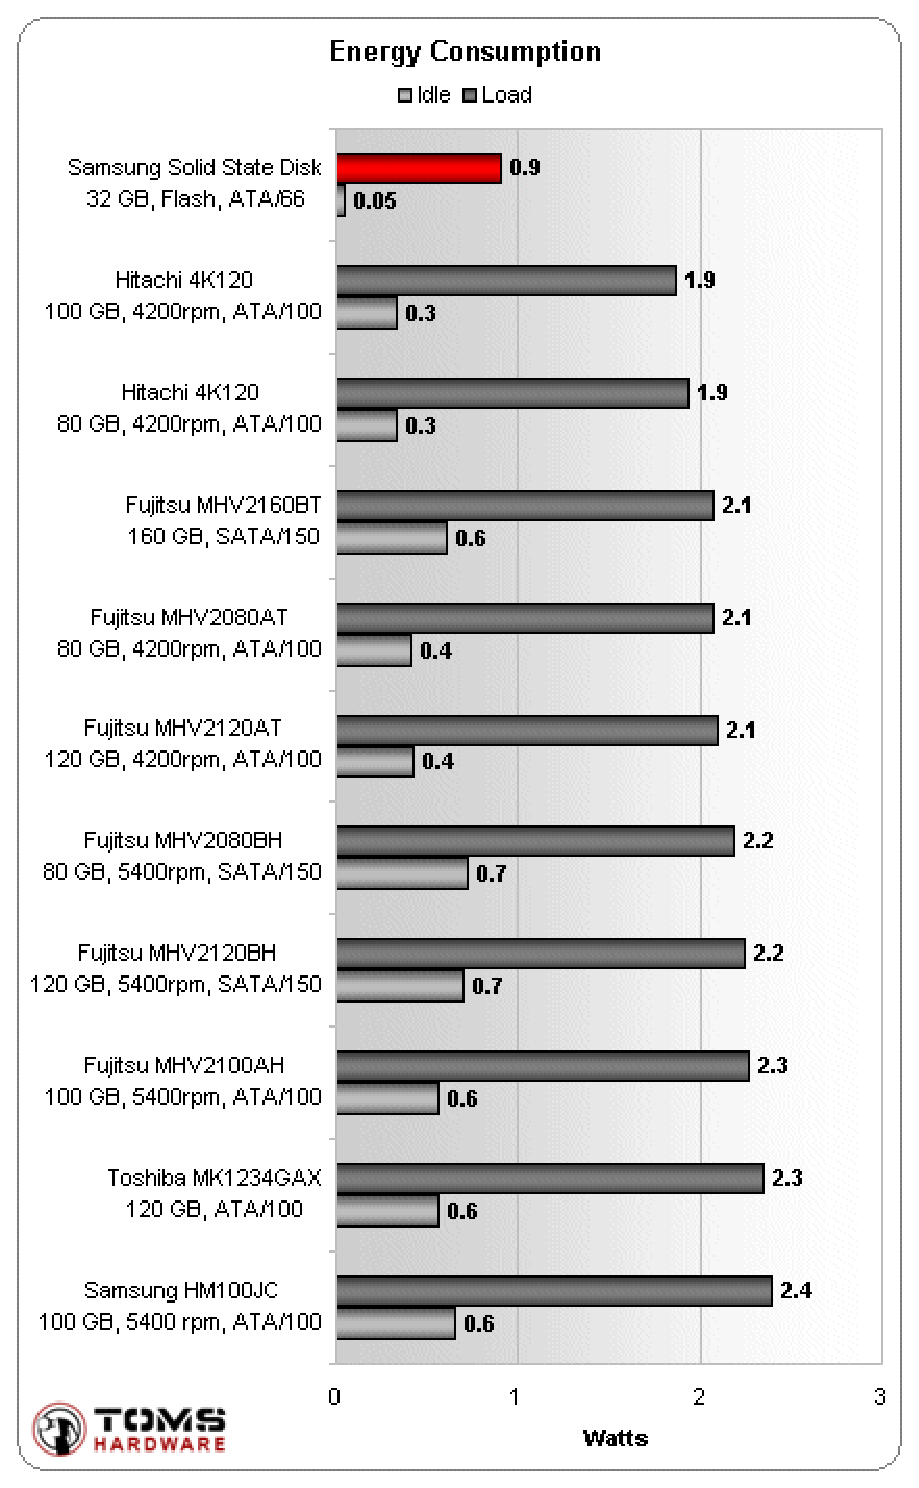
\includegraphics[scale=0.6]{graphics/power_consumption_harddrive}
                    \caption{Power Consumption for Hard-drives}
                    \label{fig:power_consumption_harddrive}
                \end{figure}
            \paragraph*{Chassis} Concerning power supply, fans or other PC components not belonging to the main parts, it is necessary to require quality other than price. Heating and cooling are really where the power consumption goes. Most computers only make up a fairly small percentage of your electrical bill. One should never underestimate the efficiency of the power supply, because most low quality ones are only about 45-55\% efficient, whereas it is possible to achieve more than 80\%.
            \paragraph*{Monitor Type} As shown by Table~\ref{tab:energy_used_monitor}\footnote{\url{http://michaelbluejay.com/electricity/computers.html}}, flat panel liquid crystal display (LCD) monitors power consumption equals to half the power of conventional CRT monitors. LCD monitors also dissipate less heat, which helps to reduce air conditioning costs. Another interesting point is that either LCD or CRT monitors consume the same amount of energy with or without screensavers. As LCD monitors do not consume much energy when turned off, that would be the best solution for idle computers.
\begin{table}[h!tb]
        \centering
        \begin{tabular}{|c|c|}
        \hline
        \multicolumn{ 2}{|c|}{{\bf Monitors}} \tnhl
        Typical 17" CRT &   80 watts \tnhl
        Typical 17" LCD &   35 watts \tnhl
        Apple MS 17" CRT$^a$ &   63 watts \tnhl
        Apple MS 17" CRT$^b$ &   54 watts \tnhl
        Screen saver$^c$ & same as above \tnhl
        Sleeping monitor$^d$ & 0-15 watts \tnhl
        Monitor turned off at switch & 0-10 watts \tnhl
        \end{tabular}  \linebreak
        $^a$ mostly white (blank IE window) \linebreak
        $^b$ mostly black (black Windows desktop with just a few icons)\linebreak
        $^c$ any image on screen\linebreak
        $^d$ dark screen
        \captionof{table}{Energy used by Monitors} 
\label{tab:energy_used_monitor}
    \end{table}

    \subsection{Policies / Tools / Labels} \label{sec2:policies_tools_labels}
        The amount of saved energy depends also on policies that regard technology acquisition and IT management, which may be enforced by a variety of specialized tools. Examples of policies that regard equipment acquisition are: the acquisition of new computers or components labeled as green by the manufacturer, purchase of computers with multi-core processors and even to discourage the purchase of specific kinds of hardware such as dual or large monitors and graphic cards. Another kind of policy relates to the management of the machines. One example of the latter is to turn off workstations or servers if they are going to be unused for a long time. This kind of measure is particularly efficient as a computer in idle mode uses 20 to 50 times the power of a computer in standby mode\footnote{\url{http://www.cosn.org/Initiatives/GreenComputing/EnergyUse/tabid/4515/Default.aspx}}.
        
    \begin{table}[h!tb]
        \centering
        \begin{tabular}{|c|c|}
        \hline
        \multicolumn{ 2}{|c|}{{\bf Computers}} \tnhl
        Desktop Computer & 60-250 watts \tnhl
        On screen Saver$^a$ & 60-250 watts \tnhl
        Sleep / Standby & 1-6 watts \tnhl
        Laptop & 15-45 watts \tnhl
        \end{tabular}\linebreak
        $^a$ no difference
        \captionof{table}{Energy used by a standard computer} 
        \label{tab:energy_used_computer}
    \end{table}

        The tools that automate these methods have as their main feature the possibility to let computers in a network in standby mode or even to turn them off after a long period of no utilization. In addition, the shared usage of networked pieces of hardware can be an effective way to achieve energy savings. Networked systems allow several nearby users to share a single printer, which generally generates savings in both equipment cost and energy if compared with each computer having a dedicated printer. Above that, choosing multifunction devices (MFD) that encapsulates in one machine the functionality of many others. In addition to saving space and materials, these multifunctionals save energy if compared to several different machines working in parallel. The Table~\ref{tab:energy_recommendation_efficient_printer}\footnote{\url{http://www1.eere.energy.gov/femp/procurement/eep_printer.html}} describes the power consumption in standby mode that an energy-efficient networked printer should have in relation to the printer type and to the number of pages it prints per minute. 
        
        \begin{table}[h!tb]
        \centering
            \begin{tabular}{|r|c|c|}
            \hline
            \multicolumn{ 3}{|c|}{{\bf Efficiency Recommendation}} \tnhl
            \multicolumn{ 1}{|c|}{Printer Speed} & \multicolumn{ 2}{|c|}{Recommended ``Sleep'' Mode$^a$} \tnhl
            \multicolumn{ 1}{|c|}{} & Laser B/W + All Ink jet$^b$ & Laser Color$^c$ \tnhl
            $\geq$10 pages/min & 10 watts or less & 35 watts or less \tnhl
            11-20 pages/min & 20 watts or less & 45 watts or less \tnhl
            21-30 pages/min & 30 watts or less & 70 watts or less \tnhl
            31-44 pages/min & 40 watts or less & 70 watts or less \tnhl
            $>$44 pages/min & 75 watts or less & 70 watts or less \tnhl
            \end{tabular}\linebreak            
            $^a$ ``Sleep'' mode is a low-power standby condition, it restores automatically with a print request.\linebreak
            $^b$ Includes both black-ink and color ink jets, and printer/fax combinations.\linebreak
            $^c$ Also includes LED and thermal transfer color printers.
            \captionof{table}{Energy Recommendation to an Energy-Efficient Printer} 
            \label{tab:energy_recommendation_efficient_printer}
        \end{table}
        
        One last kind of policy is to favor the acquisition of eco-labeled products. An eco-label is given to products that comply with some energy efficiency specifications. The most famous of these labels is the ENERGY STAR$^{\textcircled {\scriptsize R}}$, which is an energy efficiency program sponsored by the U.S. Environmental Protection Agency. For example, An ENERGY STAR$^{\textcircled {\scriptsize R}}$ qualified computer is possible to use up to 70\% less electricity than computers without enabled power management features.
            
        \subsection{Thin Client Architectures} \label{sec2:thin_clients}
            According to \emph{Wikipedia}, in 2009, ``a thin client is a client computer or client software in client-server architecture networks which depends primarily on the central server for processing activities, and mainly focuses on conveying input and output between the user and the remote server''. This is very well connected to both ideas of cloud computing and Green ICT and it is possible to subdivide in three categories for comparison against standard the PC architecture: Performance, Power Consumption and Hardware Savings and they are going to be exploited in the following subsections.
            
            \subsubsection*{PC vs. Thin Client: Performance}
                In order to analyze and give a comparison base of the performance between standard PCs and two types of thin clients, a set of tests were executed. The variable that was the number of active clients on a network, each running the same typical office applications tasks. The following client platforms were considered in this study:
                \begin{itemize}
                    \item PC: OptiPlex 210L PCs, basic managed PC desktops running Windows XP Professional;
                    \item Sun thin client: Sun Ray 2 running Sun Ray proprietary software;
                    \item Wyse thin client: Wyse Winterm 5150SE, Linux-based thin clients running Wyse Linux V6.
                \end{itemize}
                Each network used a standard file server, an HP ProLiant DL360 3.4MHz with and Intel Xeon processor and Microsoft Server 2003 Enterprise Edition. For test reasons, all the files that were manipulated by the PC were stored at the server. The tests are listed below:
                \begin{itemize}
                    \item Calculating subtotal in Microsoft Office Excel 2003 (Figure~\ref{fig:graphic_excel_test} and Table~\ref{tab:table_excel_test})
                    \item Compressing a PDF within Adobe Acrobat 7.0 Standard (Figure~\ref{fig:graphic_pdf_test} and Table~\ref{tab:table_pdf_test})
                \end{itemize}
                
                \begin{figure}[h!tb]
                    \centering
                    \resizebox{\textwidth}{!}{ % Fazendo a tabela caber no espaco da pagina
                    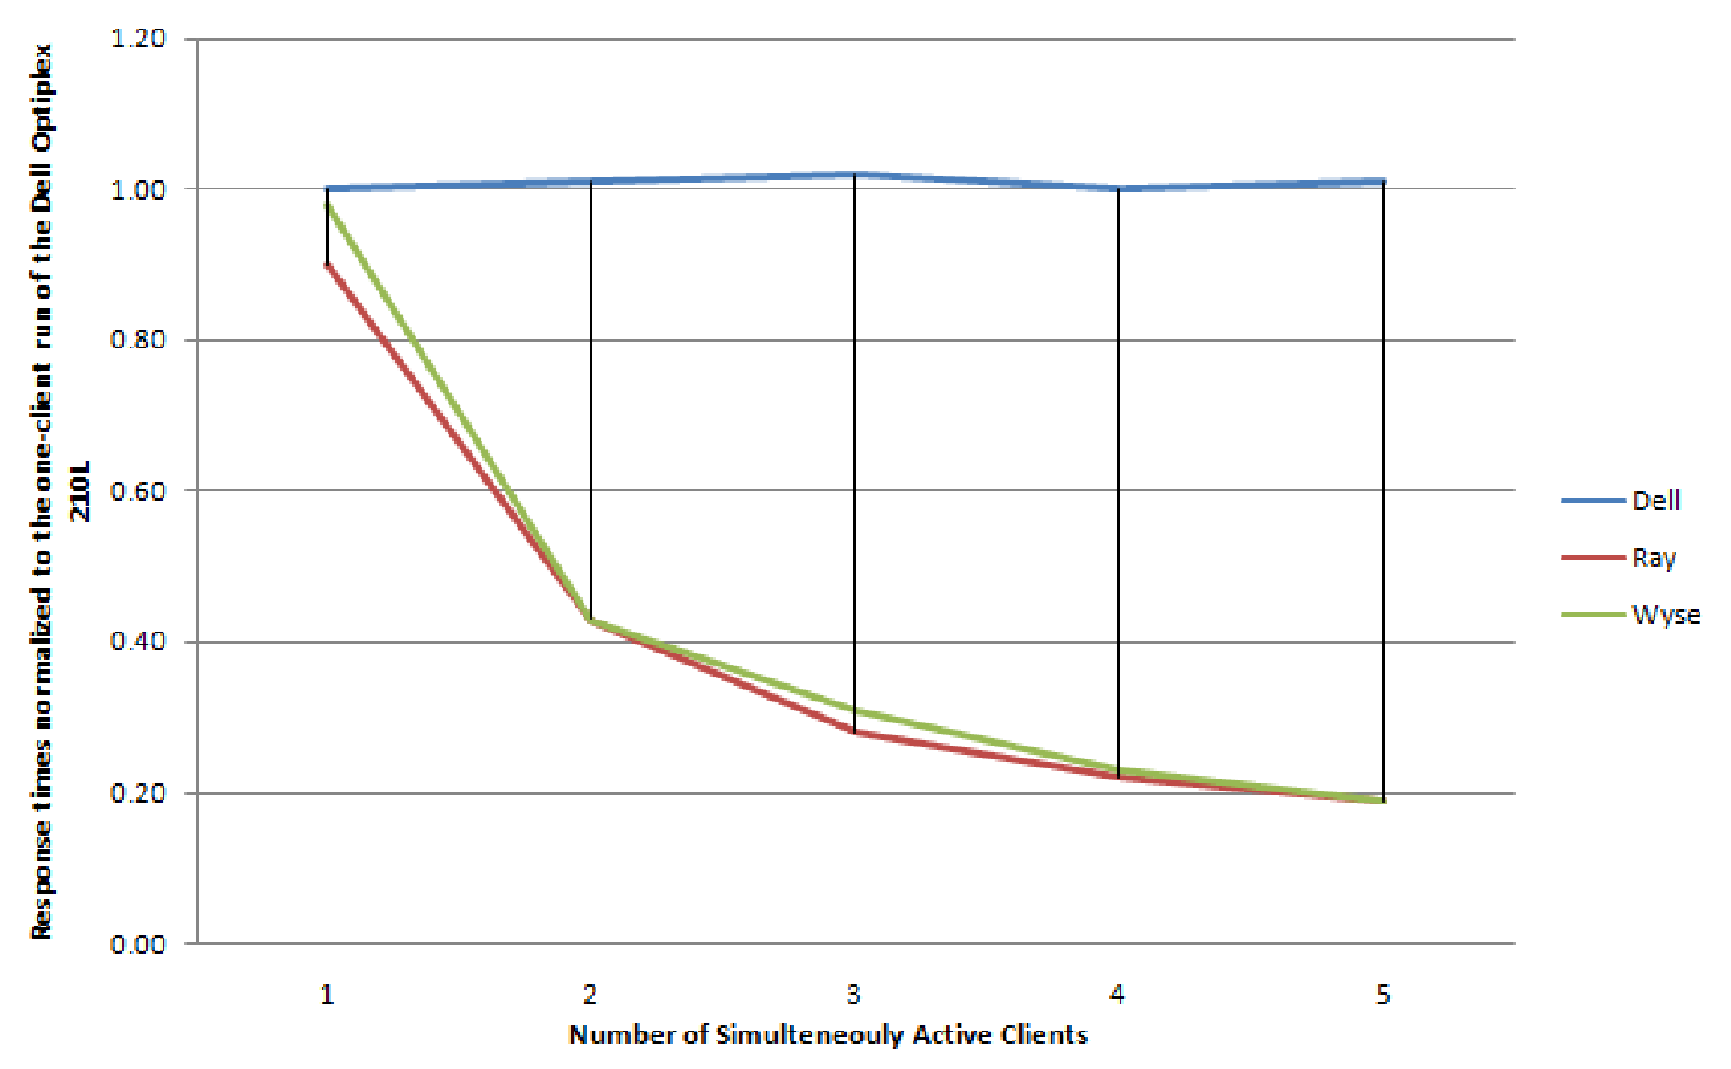
\includegraphics{graphics/graphic_excel_test}}
                    \caption{Normalized Excel Subtotals Task Response Times}
                    \label{fig:graphic_excel_test}
                \end{figure}
                \begin{table}[h!tb]
                    \centering
                    \begin{tabular}{|c|c|c|c|c|c|c|}
                    \hline
                    \multicolumn{ 3}{|c|}{Performance Results} &            & \multicolumn{ 3}{|c|}{Comparative Rating} \tnhl
                    PC solution & \multicolumn{ 2}{|c|}{Thin-client solutions} & Number of   & PC solution & \multicolumn{ 2}{|c|}{Thin-client solutions} \tnhl
                          Dell &        Sun &       Wyse & concurrent &       Dell &        Sun &       Wyse \tn

                      OptiPlex &        Ray &    Winterm &     active &   OptiPlex &        Ray &    Winterm \tn

                          210L &          2 &     5150SE &    clients &       210L &          2 &     5150SE \tnhl
                          12.9 &       13.2 &       13.1 &          1 &       1.00 &       0.90 &       0.98 \tnhl
                          12.8 &       30.2 &       29.7 &          2 &       1.01 &       0.43 &       0.43 \tnhl
                          12.7 &       45.5 &       41.9 &          3 &       1.02 &       0.28 &       0.31 \tnhl
                          12.9 &       58.3 &       57.3 &          4 &       1.00 &       0.22 &       0.23 \tnhl
                          12.8 &       68.1 &       67.9 &          5 &       1.01 &       0.19 &       0.19 \tnhl
                    \end{tabular}  
                    \captionof{table}{Performance Results for Excel Subtotals Calculation} 
                    \label{tab:table_excel_test}
                \end{table}
                \begin{figure}[h!tb]
                    \centering
                    \resizebox{\textwidth}{!}{ % Fazendo a tabela caber no espaco da pagina
                    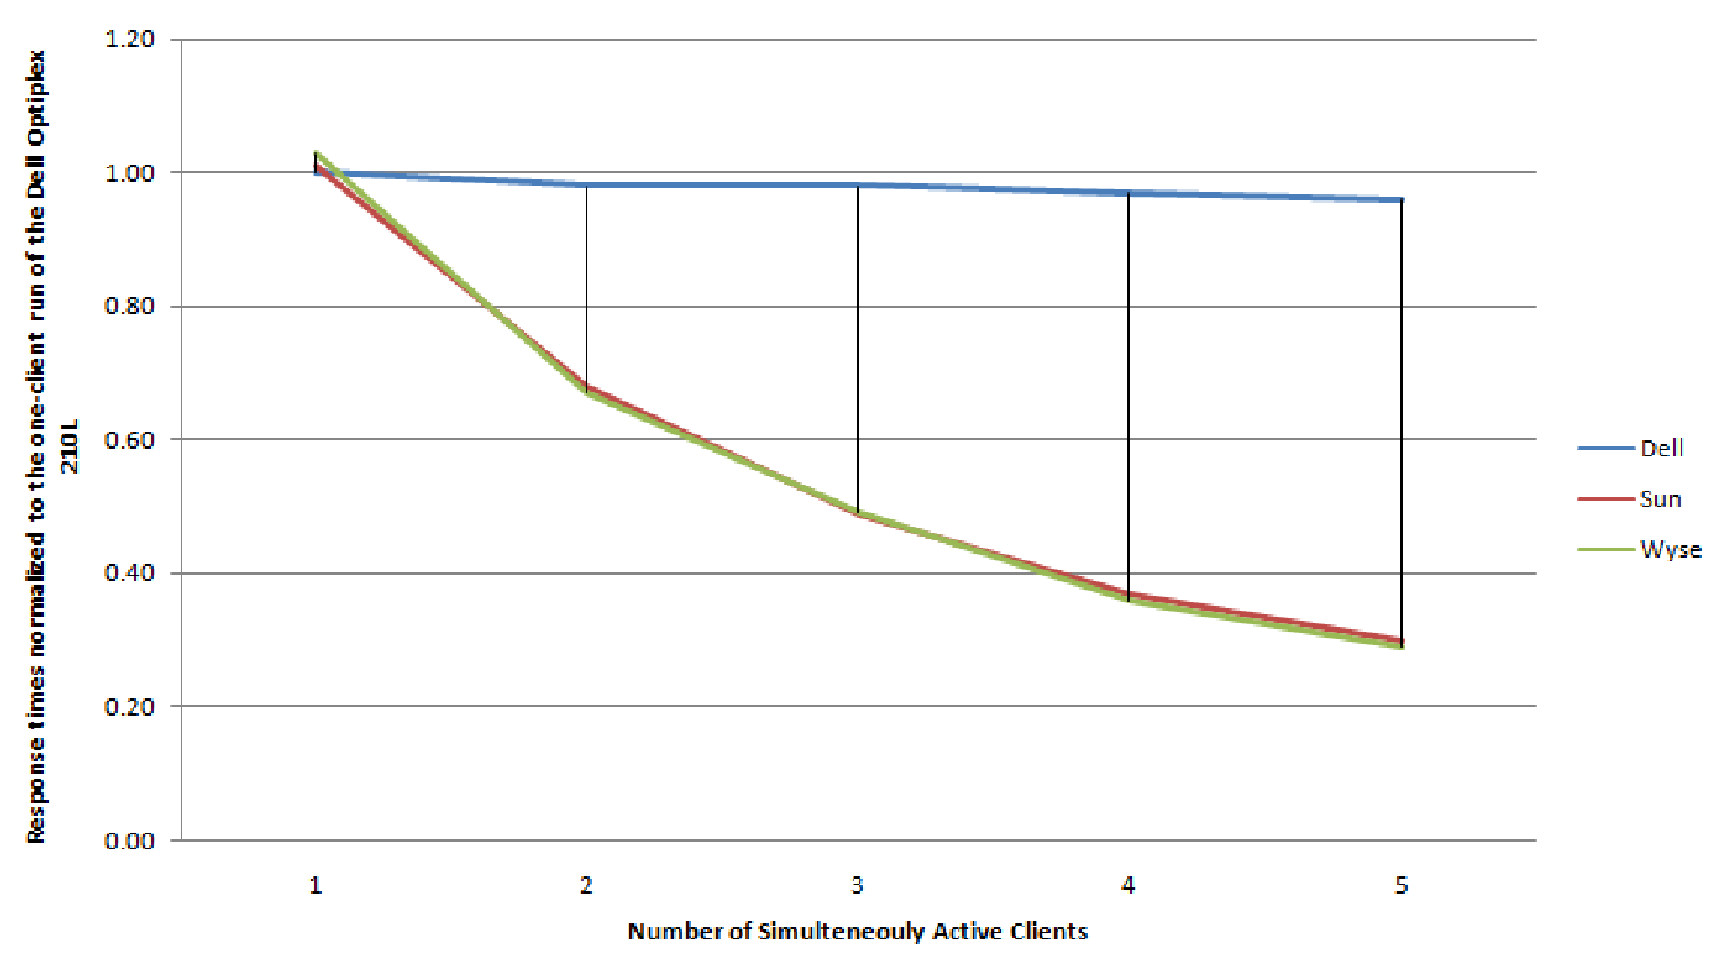
\includegraphics{graphics/graphic_pdf_test}}
                    \caption{Normalized PDF Subtotals Task Response Times}
                    \label{fig:graphic_pdf_test}
                \end{figure}
                \begin{table}[h!tb]
                    \centering
                    \begin{tabular}{|c|c|c|c|c|c|c|}
                    \hline
                    \multicolumn{ 3}{|c|}{Performance Results} &            & \multicolumn{ 3}{|c|}{Comparative Rating} \tnhl
                    PC solution & \multicolumn{ 2}{|c|}{Thin-client solutions} & Number of   & PC solution & \multicolumn{ 2}{|c|}{Thin-client solutions} \tnhl
                        Dell   &        Sun &       Wyse & concurrent &     Dell   &        Sun &       Wyse \tn

                      OptiPlex &        Ray &    Winterm &     active &   OptiPlex &        Ray &    Winterm \tn

                          210L &          2 &     5150SE &    clients &       210L &          2 &     5150SE \tnhl
                          16.1 &       16.0 &       15.6 &          1 &       1.00 &       1.01 &       1.03 \tnhl
                          16.4 &       23.8 &         24 &          2 &       0.98 &       0.68 &       0.67 \tnhl
                          16.5 &       33.0 &       33.1 &          3 &       0.98 &       0.49 &       0.49 \tnhl
                          16.6 &       43.7 &       44.3 &          4 &       0.97 &       0.37 &       0.36 \tnhl
                          16.7 &       54.0 &       55.1 &          5 &       0.96 &       0.30 &       0.29 \tnhl
                    \end{tabular}  
                    \captionof{table}{Performance Results for PDF Compression Subtotals Calculation}
                    \label{tab:table_pdf_test}
                \end{table}
                \pagebreak
            \subsubsection*{PC vs. Thin Client: Power Consumption}
                Supposing 30 thin users share a 400W server, the total power consumption will be 1300W - a yearly cost of \euro640.00. 30 PCs would consume 10000W instead - a yearly cost of \euro4900.00 (assuming the MWh cost is \euro80.00). The Table~\ref{tab:pc_thin_client_power_consumption} shows the power consumption of thin-client and PC.
                \begin{table}[h!tb]
                \centering
                    \begin{tabular}{|c|c|c|}
                    \hline
                         & {\bf Thin Client} &   {\bf PC} \tnhl
                    {\bf Weight} & 2.2 - 7.7 lbs & 22 - 33 lbs \tnhl
                    {\bf Volume} & 1.5 - 3 dm$^3$ & 30 - 35 dm$^3$ \tnhl
                    {\bf Packing material} & 2.2 - 4.4 lbs &   3 - 5 kg \tnhl
                    {\bf Power consumption\linebreak (including monitor)} & 20 - 50 watt & 300 - 400 watt \tnhl
                    {\bf Heat rejection} & 5 - 35 watt & 85 - 115 watt \tnhl
                    {\bf Noise level} & 0 dbA & 50 - 60 dbA \tnhl
                    \end{tabular}  
                    \captionof{table}{PC and thin client power consumption} 
                    \label{tab:pc_thin_client_power_consumption}
                \end{table}
                
            \subsubsection*{Hardware Savings}
                \paragraph*{Savings on client hardware} 
                    The economy brought by the substitution of PCs with thin clients was estimated around US\$ 208 per PC per year. The estimative considered the average prices of a PC, an adequate thin client and the PC upgrade costs every 3 years. If energy consumption is considered, the savings will be even greater.

                The following considerations were taken:
                \begin{itemize}
                    \item Thin client cost: US\$250.00 x PC cost: US\$750.00;
                    \item PC needs to be upgraded every 3 years and thin clients need to be replaced every 6 years.
                \end{itemize}
                Therefore, in a 6-year period US\$1500.00 will be spent on a PC against US\$250.00 that will be spent on a thin client.

            \paragraph*{Extra server hardware costs}
                Considering that:
                \begin{itemize}
                    \item On average 30 users will need a dual processor server with 4 GB of RAM and SCSI hard disks;
                    \item A brand new server should cost around US\$4,500.00 and will depreciate on average in 3 years.
                \end{itemize}
                For 60 users, the thin client solution should out-price the PC one by US\$11,300.00 per year, excluding the administration costs of both solutions.

        \subsection{Servers and Virtualization} \label{sec2:servers_virtualization}
                        
            \subsubsection*{Rack vs. Blade}
                According to Goldworm\cite{barbAnne07}, Blade servers are a package of ``ultra-high density components including servers, storage, and communications interfaces in a pre-wired chassis with shared components such as power, cooling, and networking. In contrast to the conventional \emph{horizontal} positioning within a rack (rack mounted servers), blades servers are typically (though not always) installed \emph{vertically} in a blade chassis, like books in a bookshelf''. This disposition of the blade servers along with their reduced dimension provide a high server density and thus of performance. For example, 60 blade servers such as the one depicted in Figure~\ref{fig:example_blade_server} can fit in the same physical space as 42 rack-mounted servers. A blade enclosure, which can hold from 8 to 24 \cite{Rehn08} blade servers, provides common services such as power supply, cooling and networking thus eliminating redundancies in each individual blade server. A standard rack can accommodate more than 250 blade servers against approximately 42 standard servers.
            \begin{figure}[h!tb]
                \centering
                \subfloat[IBM LS20]{
                    \label{fig:ibm_ls20_blade_server}
                    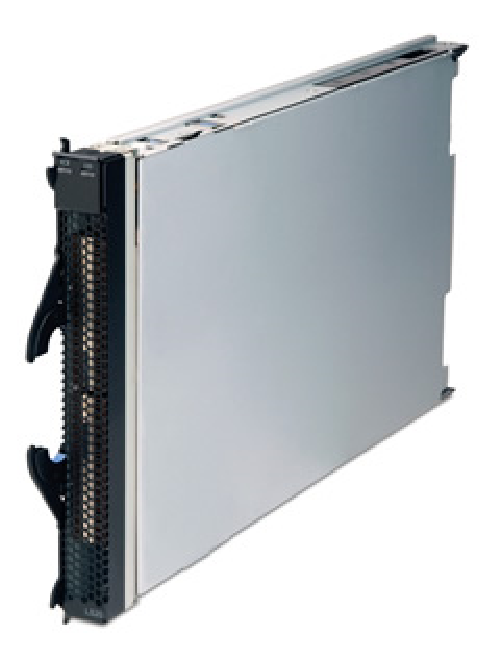
\includegraphics[width=0.3\textwidth]{graphics/ibm_ls20_blade_server}}
                \subfloat[Sun 6000 Series Blade Enclosure]{
                    \label{fig:sun_6000_blade_enclosure}
                    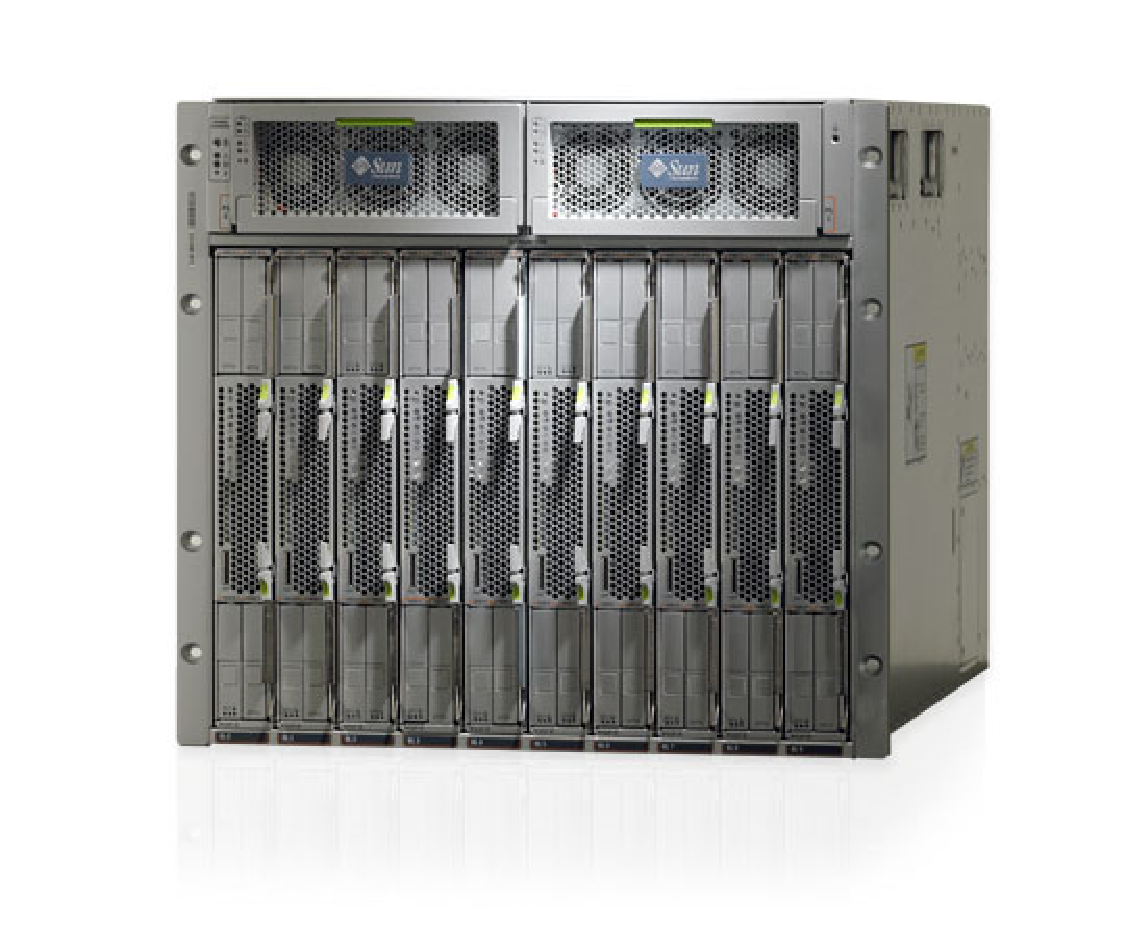
\includegraphics[width=0.3\textwidth]{graphics/sun_6000_blade_enclosure}}
                \subfloat[HP Intros Rack]{
                    \label{fig:hp_intros_blade_server_rack}
                    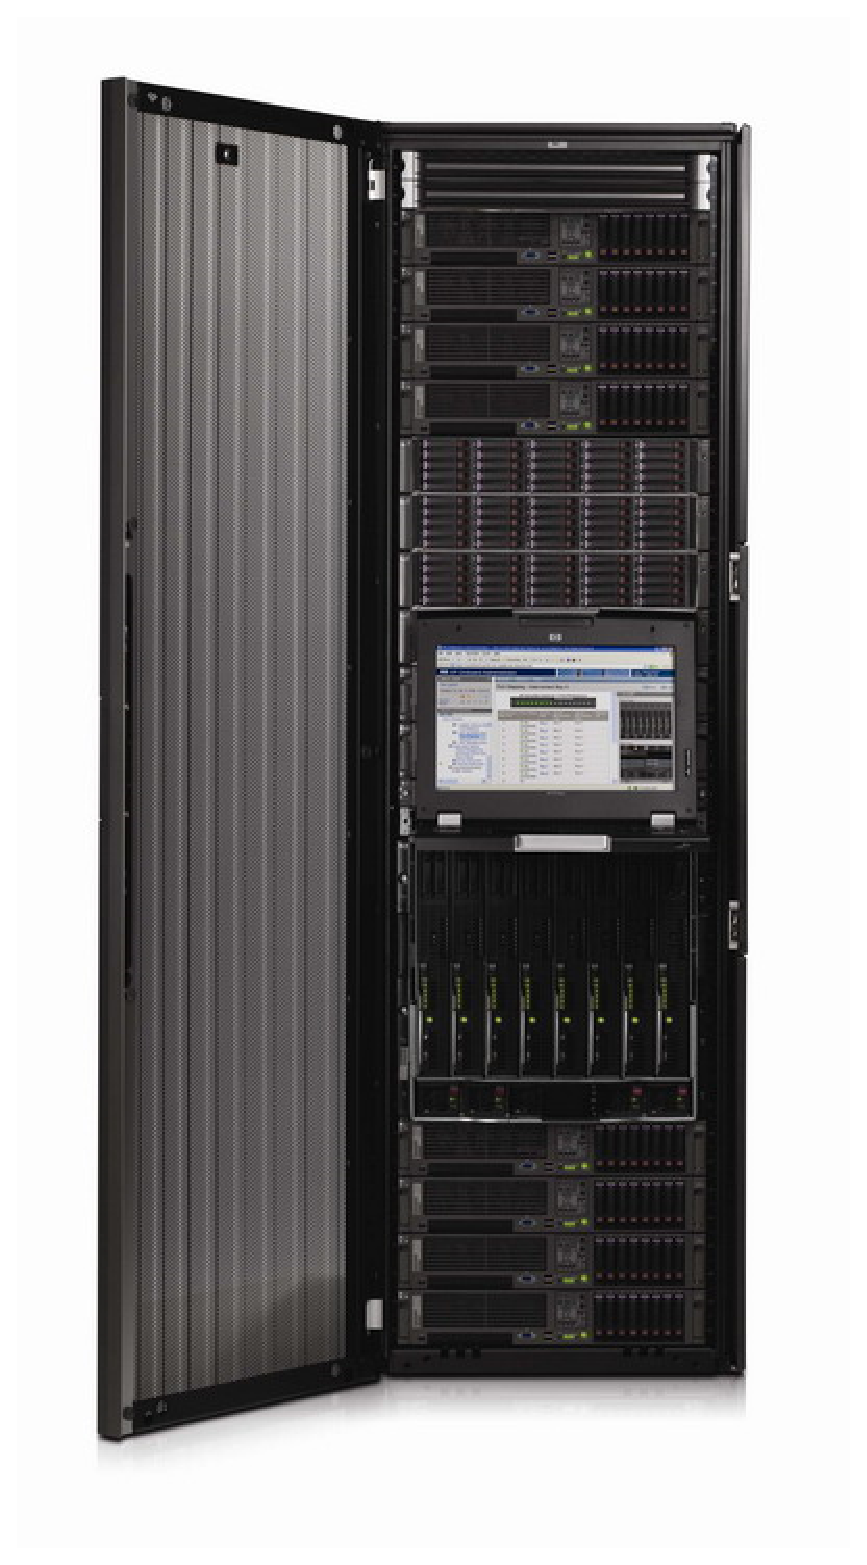
\includegraphics[width=0.3\textwidth]{graphics/hp_intros_blade_server_rack}}
                \caption{Examples of Blade Servers}
                \label{fig:example_blade_server}
            \end{figure}
            \begin{figure}[h!tb]
                \centering
                \subfloat[Chenbro 5U RM51924]{
                    \label{fig:chenbro_5urm51924}
                    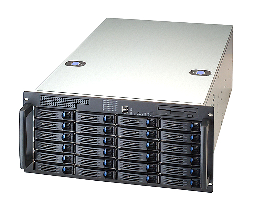
\includegraphics[width=0.3\textwidth]{graphics/chenbro_5U_RM51924}}
                \subfloat[Rack Server]{
                    \label{fig:rack_server}
                    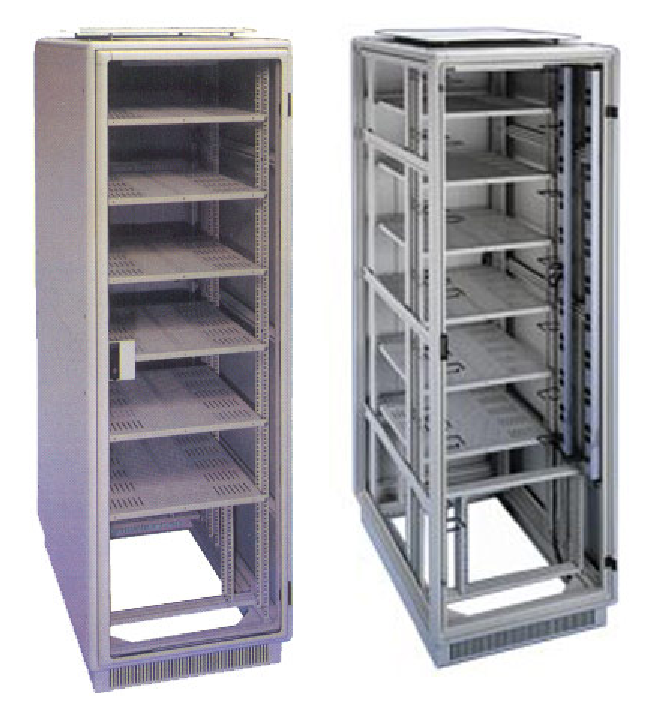
\includegraphics[width=0.3\textwidth]{graphics/rack_server}}
                \caption{Examples of Rack Servers}
                \label{fig:example_rack_server}
            \end{figure}
            In the Table~\ref{tab:power_consumption_several_servers}, a comparison is made between IBM HS21 blades and x3550 rack servers. The blades and rack servers have comparable performance.
            \begin{itemize}
                \item 2.0 GHz intel quad core;
                \item 8 GB DDR2 memory;
                \item Both in standard configuration, with no HDDs.
            \end{itemize}
            \begin{table}[h!tb]
                \centering
                \begin{tabular}{|c|c|c|c|}
                \hline
                \multicolumn{ 1}{|c|}{{\bf IBM server model}} & \multicolumn{ 1}{|c|}{{\bf Base Power}} & \multicolumn{ 1}{|c|}{{\bf kWh consumed}} & \multicolumn{ 1}{|c|}{{\bf Total cost }} \tn
                \multicolumn{ 1}{|c|}{{\bf }} & \multicolumn{ 1}{|c|}{{\bf Consumption}} & \multicolumn{ 1}{|c|}{{\bf over 5 years}} & \multicolumn{ 1}{|c|}{{\bf (\$0.03/kWh)}} \tn
                \multicolumn{ 1}{|c|}{{\bf }} & \multicolumn{ 1}{|c|}{{\bf }} & \multicolumn{ 1}{|c|}{{\bf }} & \multicolumn{ 1}{|c|}{{\bf over 5 years}} \tnhl
                BC-H Chassis, no blades & 0.510 kWh &     22,350 &  \$670.50  \tnhl
                BC-H HS21 blade & 0.318 kWh &     13,936 &  \$418.08  \tnhl
                x3550 server & 0.373 kWh &     16,346 &  \$490.39  \tnhl
                x3650 server & 0.455 kWh &     19,940 &  \$598.20  \tnhl
                BC-H chassis with 14 & 4.962 kWh &    217,455 & \$6,523.65  \tn
                HS21 blades &  &  &  \tnhl
                14 x3550 servers & 5.222 kWh &    228,849 & \$6,865.46 \tnhl
                14 x3650 servers & 6.370 kWh &    279,259 & \$8,374.80  \tnhl
                \end{tabular}  
                \captionof{table}{Power consumption for several servers, excluding cooling and redundancy}%XXX colocar referencia
                \label{tab:power_consumption_several_servers}
            \end{table}

            \begin{itemize}
                \item Space saving and efficiency - packing more computer power in a significantly smaller area;
                \item Consolidation of servers to improve and centralize management as well as utilization;
                \item Return on investment (ROI) and improved total cost of ownership (TOC) through increased hardware utilization and reduced operating expenses;
                \item More energy efficient, due to existence of centralized power supply, cooling and networking.
            \end{itemize}
            According to the figures, the choice of using a blade server provides roughly 5\% power saving over a similar rack-mount configuration. The main benefit brought by the use of blade servers, however, is the processing density, as a rack filled with blade servers may carry up to 50\% more servers than one with rackable servers. Other benefits are that blade servers are easier to service and reduce the number of power cables needed from as much as 80\% \cite{Hendenson07}. 
            
            In conclusion, blade servers do not provide much in terms of power saving but it greatly reduces the amount of space used in datacenters. However, the high power density might prove to be a problem to server farms in terms of overheating. Solutions to this problem are described in the section of Data Center Infrastructure.
            
            \subsubsection*{Virtualization}
                The overall goal of virtualization is to create a logical abstraction of physical assets. It allows multiple ``virtual'' servers to run on one physical server, thereby consolidating many physical servers into one. \emph{Wikipedia}, in 2009, defines virtualization as the following: ``Virtualization is the process of presenting a logical grouping or subset of computing resources so that they can be accessed in ways that give benefits over the original configuration. This new virtual \emph{view} of the resources is not restricted by the implementation, geographic location or the physical configuration of underlying resources.''. Virtualization can improve efficiency and availability of resources and applications in the organization and according to \emph{Vmware}, the choice of virtualized servers over the standard nonvirtualized configuration makes possible to save 50-70\% overall IT costs. Apart from the reduction of costs, virtualization may free up IT resources, provide better infrastructure optimization and utilization, increase availability and improve desktop management.
                
                Besides that, virtualization has made positive improvements to the environment issue. Gartner \cite{GartnetStamford07} estimates that 1.2 million workloads run in virtual machines, which represents an annual aggregate power savings of about 8.5 billion kWh - more electricity than is consumed annually in all of New England for heating, ventilation and cooling. While this is a good start, there are plenty of opportunities for saving even more energy and money. Analyst firm IDC \cite{IDCDoc07} states that the un-utilized server capacity equates to approximately:
                \begin{itemize}
                    \item in term of equipment and energy costs : US\$140 billion annually
                    \item in terms of hardware costs : 3 years supply of hardware
                    \item in terms of computing power : more than 20 million servers 
                \end{itemize}
                At the annual production rate of 4 tons of carbon dioxide (CO$_{2}$) per server, these un-utilized servers produce a total of more than 80 million tons of CO$_{2}$ per year. This is more than is emitted from the country of Thailand and more than half of all countries in South America. From the organizational point of view these data suggests that virtualization is a good improvement to the data center, saving not only space provided to the servers but also saving energy by reducing the idle time of the servers and augmenting their workload. It is also important to state that, by providing a virtualized solution, the number and variety of available applications can be increased.
                
                There are two kinds of virtualization that may be used in a data center: storage and computing virtualization. Storage-area networks (SAN) may be implemented to present several different physical storage racks as a single virtual storage pool \cite{Antonopoulos05}. On the other hand, computing virtualization can be implemented in two ways. The first case is when a single physical server can offer multiple virtual servers, each with its own OS. Another option is to consolidate multiple physical servers into a cluster that acts as a single server. There are cross-platform server virtualization softwares available which allows data center managers to cluster and partition servers.
                \begin{figure}[h!tb]
                    \centering
                    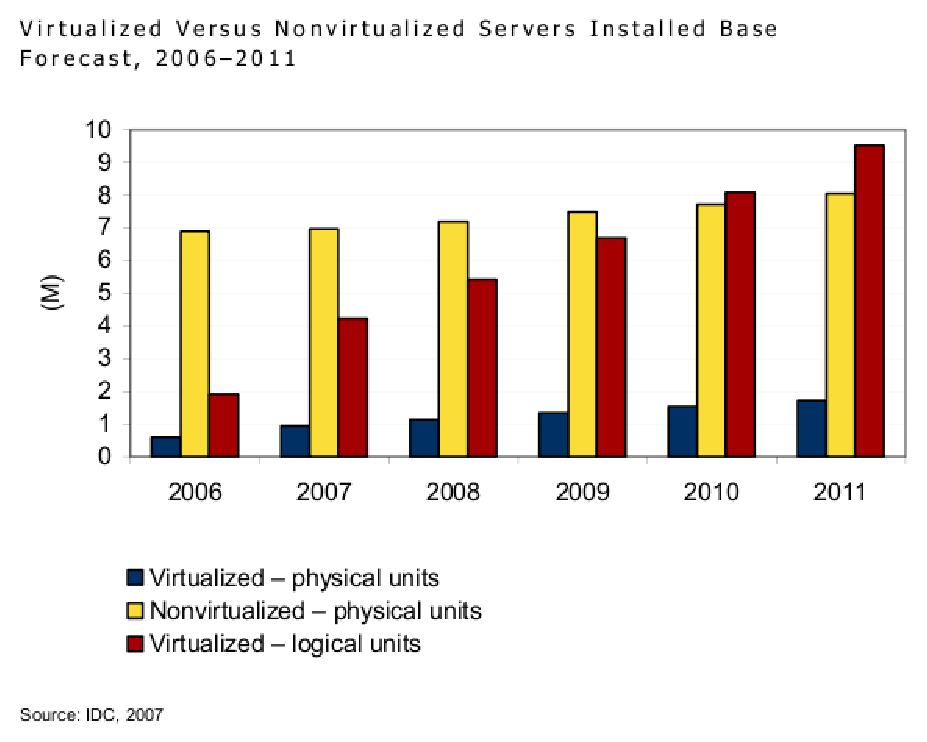
\includegraphics{graphics/installed_base_virtualized_servers}
                    \caption{Installed Base of Virtualized and Non-Virtualized Servers}
                    \label{fig:installed_base_virtualized_servers}
                \end{figure}
                
                According to the Figure~\ref{fig:installed_base_virtualized_servers} there is a trend indicating an increasing number of virtualized units over time along a forecast that by the end of 2009 the number of virtualized servers will be greater than non-virtualized ones. Logical units represent virtualized storage while physical units represent the use of non-virtualized storage. As shown in the Figure~\ref{fig:illustration_virtualization_to_physical_server}, virtualization tools such as VMware allow one physical server to act as a number of logical servers. VMware also provides a benchmark tool called VMmark\footnote{\url{http://www.vmware.com/products/vmmark/}} along with a set of test results in \cite{Makhija06} for a configuration that includes a mail server, a java server, a standby server, a web server, a database server and a file server.
                \begin{figure}[h!tb]
                    \centering
                    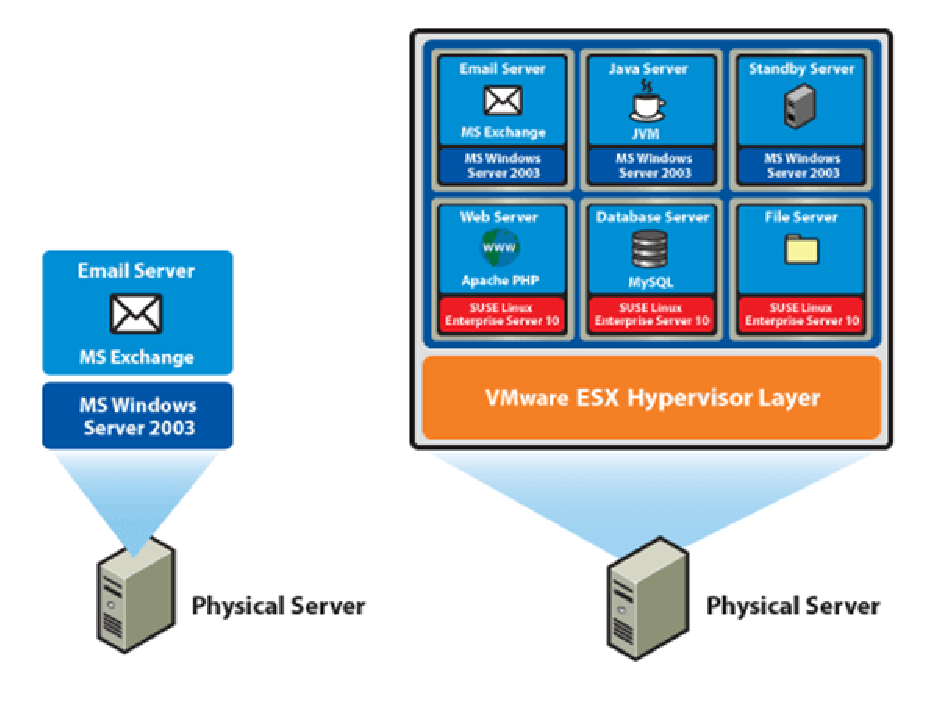
\includegraphics[scale=0.7]{graphics/illustration_virtualization_to_physical_server}
                    \caption{Illustration of Virtualization Applied to a Physical Server}
                    \label{fig:illustration_virtualization_to_physical_server}
                \end{figure}
                
                Coming along with the virtualization trend are high-throughput and eco-responsible processors such as the Sun's UltraSPARC T1 processor \cite{Hetherington05}, which support up to 128 virtualized systems in a single server and gives one of the best performance per watt of the available processors. As shown in the Table~\ref{tab:performance_power_dissipation_several_processors}\footnote{\url{http://www.anandtech.com/cpuchipsets/showdoc.aspx?i=2657&p=4}}, with relation to the UltraSPARC CPU the only comparable performance was met by the POWER5+ processor, which in average dissipates 4.5 times as much as the earlier.
                \begin{table}[h!tb]
                    \centering
                    \begin{tabular}{|c|c|c|c|c|c|c|}
                    \hline
                          &            & {\bf Power}       &                & {\bf Number}  &           &  \tn
                        &            & {\bf Dissipation} &                & {\bf of}      &           &  \tn
                        &            & {\bf CPUs}        & {\bf Number}   & {\bf Active}  & {\bf Score}   & {\bf Score} \tn
                  {\bf System} & {\bf CPU} & {\bf (Estimated)} & {\bf of cores} & {\bf Threads} & {\bf (bops)} & {\bf (\%)} \tnhl
                    Sun Fire  &  1x 1.2GHz &    72-79 W &          8 &         32 &     63.378 &      160\% \tn
                    T2000 & UltraSPARC T1 &            &            &            &            &            \tnhl
                    Sun Fire  &  2x 2.4GHz &  150-180 W &          4 &          4 &     45.124 &      114\% \tn
                    X4200 & DC Opteron &            &            &            &            &            \tnhl
                    IBM &  2x 1.9GHz &  320-360 W &          4 &          8 &     61.789 &      156\% \tn
                    p5 550 &    POWER5+ &            &            &            &            &            \tnhl
                    IBM 346 & 2x 2.8GHz  &  270-300 W &          4 &          8 &     39.585 &      100\% \tn
                    xSeries &    DC Xeon &            &            &            &            &            \tnhl
                    \end{tabular}
                    \captionof{table}{Performance and Power Dissipation for Several Processors by the Specjbb2005 Java Benchmark}
                    \label{tab:performance_power_dissipation_several_processors}
                \end{table}
                
        \subsection{Data Storage} \label{sec2:data_storage}
            There are currently three main technologies to store data: hard disks, tape drives and flash-based storage. This session will cover the first two, as they are the predominant technologies in datacenters. At the end of the session a comparison will be made between hard and tape drives.
            
            \subsubsection*{Tape Drives}
                A tape drive is a data storage device that reads and writes data stored on a magnetic tape. Its main use is as archival storage of data stored in hard drives. It is typically used for archival storage of data stored on hard drives. 
Tape media generally has a favorable unit cost, long archival stability and low energy consumption per MB of data stored to compensate for their slow seek times. Despite the slow seek time, tape drives can stream data to tape as quickly as hard drives. For example, modern LTO drives can reach continuous data transfer rates of up to 80MB/s, which is as fast as most 10,000rpm hard disks, according to \emph{Wikipedia, 2008}. Tape drives can range in capacity from a few megabytes to hundreds of gigabytes. Data can be compressed as to maximize the capacity usage. In this case the compression rate is of usually 2:1. A set of tables related to tape drives can be found in Appendix~\ref{app:comparison_tape_drives}
            
            \subsubsection*{Disk Arrays}
                Disk array refers to a linked group of one or more physical independent hard disks constituting a larger, high-performance system. They are usually implemented using RAID technology, which can provide component redundancy and high throughputs.
        
            \subsubsection*{Comparison between Tape Drives and Disk Arrays}
                Supposing a 995 TB database consisting of:
                \begin{itemize}
                	\item Storage base (frequently used data)
                	\item Backup cache (13 weeks)
                	\item Backup archive (1 year backup)
                \end{itemize}
                A solution consisting exclusively of disk arrays would require four 32-drawer disk array systems of 245 TB each. In order to ensure reliability and recoverability, a RAID5 format with two RAID5 arrays assigned to each drawer has been assumed. The total equipment cost is estimated on US\$10.57M \cite{Reine08} and according to the following table the disk array solution consumes 98KWh per TB per year.
                \begin{table}[h!tb]
                \centering 
                \resizebox{\textwidth}{!}{ % Fazendo a tabela caber no espaco da pagina
                \begin{tabular}{|c|c|c|c|c|c|c|c|c|}
                \hline
                & & {\bf Standby} & {\bf Per} & {\bf Number} & {\bf Total} & {\bf Power} &  & {\bf Annual} \tn
                & {\bf Processor} & {\bf Power} & {\bf SATA} & {\bf of SATA} & {\bf Array} &  {\bf Per} & {\bf Annual} & {\bf Cost} \tn
                {\bf Power} & {\bf Chassis} & {\bf Supply} & {\bf Drawer} & {\bf Drawers} & {\bf Power} &  {\bf Day} & {\bf Power} & US\$0.12/kWh \tnhl
                {\bf Typical} &  430 W/h &  34 W/h &  325 W/h &   32 &  11 kW/h & 264 kWh & 96,360 kWh & 11,563 \tnhl
                {\bf Maximum} &  800 W/h &  300 W/h &  425 W/h &   32 &  15 kW/h & 360 kWh & 131,400 kWh &  15,768 \tnhl
                \end{tabular}}
                \captionof{table}{Tape Drive Power Costs}%XXX verificar nome da tabela
                \label{tab:tape_drive_power_costs} %XXX verificar nome da tabela
                \end{table}
                With a native capacity of 800GB and throughput of 120 MB/sec, an LTO 4 drive has a compressed capability to write at 240 MB/sec, or 864 GB/hour. Supposing the same database is to be entirely stored at this drive, the equipment cost would be of US\$233,878.00 with an annual energy cost of US\$599.00.The tape solution will consume 1150 kWh in 1 year or 1,16kWh per TB per year.
                \begin{table}[h!tb]
                \centering 
                \resizebox{\textwidth}{!}{ % Fazendo a tabela caber no espaco da pagina
                \begin{tabular}{|c|c|c|c|c|c|c|c|c|}\hline
                {\bf N$^o$ of  } & {\bf N$^o$ of } & {\bf Library } & {\bf Frame} & & {\bf Drive} &  &   &  \tn
                {\bf frames} & {\bf drives } & {\bf acquisition } & {\bf acquisition } & {\bf Cartridge } & {\bf acquisition } & {\bf Space} & {\bf Energy} & {\bf Total} \tn
                {\bf acquired} & {\bf acquired} & {\bf cost} & {\bf cost} & {\bf cost} & {\bf cost} & {\bf cost} & {\bf cost} & {\bf cost} \tnhl
                1 &    2 &    76,000 &    30,000 &   82,278 &   45,600 &   68,850 &   599 &    303,327 \tnhl
                \end{tabular}}
                \captionof{table}{Disk Array Power Costs}%XXX verificar nome da tabela
                \label{tab:disk_array_power_costs} %XXX verificar nome da tabela
                \end{table}
                In overall, for the 995 TB database the following conclusions can be drawn:
                \begin{itemize}
	                \item Disk arrays consume 84 times as much as tape drives, per TB stored
	                \item The disk array solution costs 35 times as much as the tape drive solution
                \end{itemize}
                Although the cost difference between of both solutions may be high, performance should be also considered in the comparison. In that case, an adequate proportion between disk array and tape storage must be drawn according to the frequency of backup access.

        \subsection{Power Architectures} \label{sec2:power_architectures}
            \subsubsection*{Conventional AC Architecture}
                \begin{figure}[h!tb]
                    \centering
                    \resizebox{\textwidth}{!}{ % Fazendo a tabela caber no espaco da pagina
                    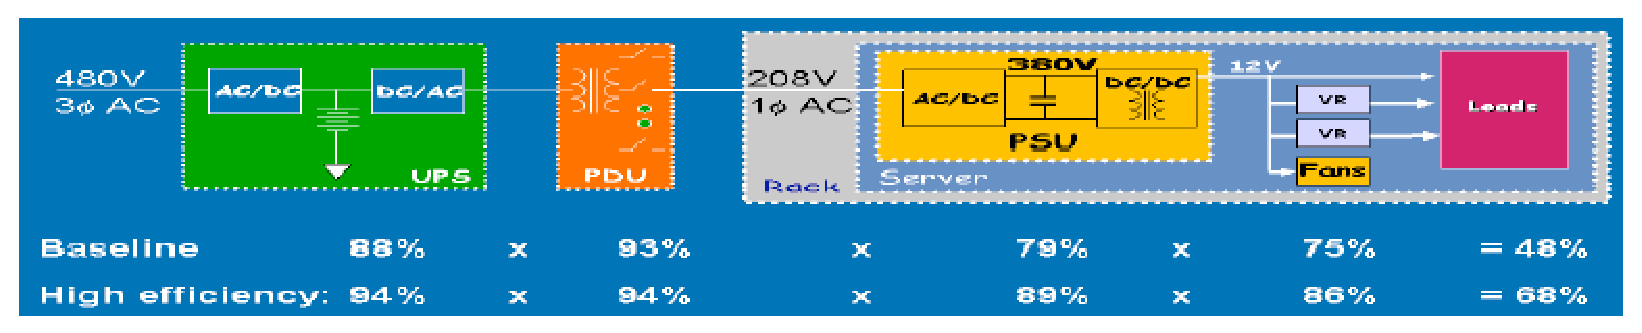
\includegraphics{graphics/conventional_ac_efficiency}}
                    \caption{Conventional AC architecture efficiency}
                    \label{fig:conventional_ac_efficiency}
                \end{figure}
                In this configuration (Figure~\ref{fig:conventional_ac_efficiency}) the following transformations take place:
                \begin{itemize}
	                \item PDU steps down the voltage from 480VAC to 208VAC;
                    \item Power Supply Unit (PSU) converts 208VAC to 380VDC;
                    \item Final component distribution at 12VDC.
                \end{itemize}
                The efficiency is measured for both conventional (baseline) and high efficiency (best-in-class) equipments. The difference in efficiency between the two equipment choices is of 20\%.

            \subsubsection*{Rack-Level DC Architecture}
                \begin{figure}[h!tb]
                    \centering
                    \resizebox{\textwidth}{!}{ % Fazendo a tabela caber no espaco da pagina
                    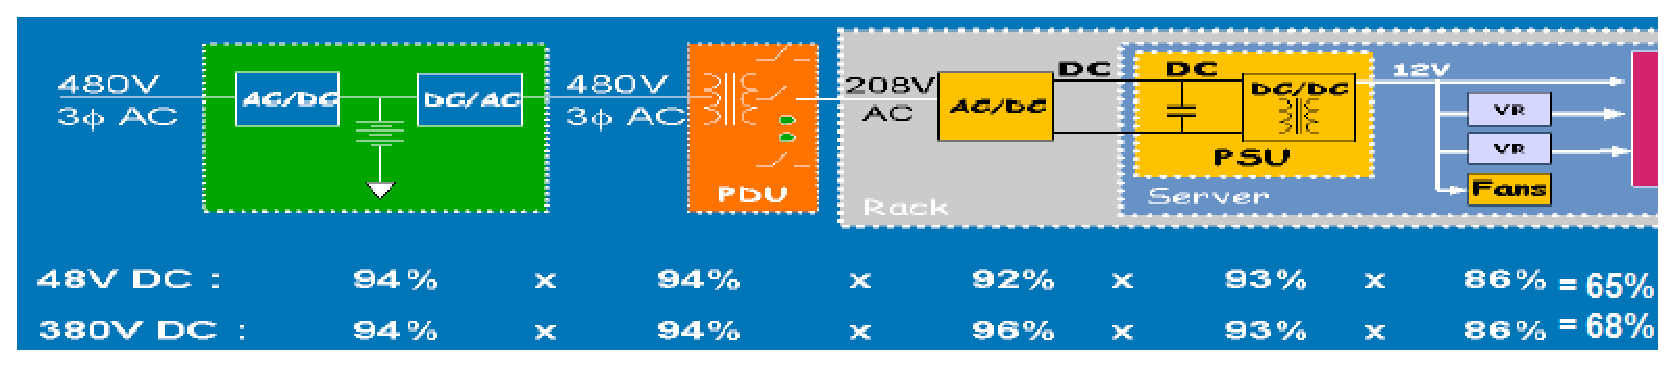
\includegraphics{graphics/rack_level_dc_efficiency}}
                    \caption{Rack-level DC architecture efficiency}
                    \label{fig:rack_level_dc_efficiency}
                \end{figure}
                On Figure~\ref{fig:rack_level_dc_efficiency}, it is possible to see that, after the PDU, an 208VAC to 48VDC/380VDC conversion is made in the rack. PSU and PDU are considered to be best-in-class, with high efficiency.

            \subsubsection*{Facility-level DC Architecture}
                \begin{figure}[h!tb]
                    \centering
                    \resizebox{\textwidth}{!}{ % Fazendo a tabela caber no espaco da pagina
                    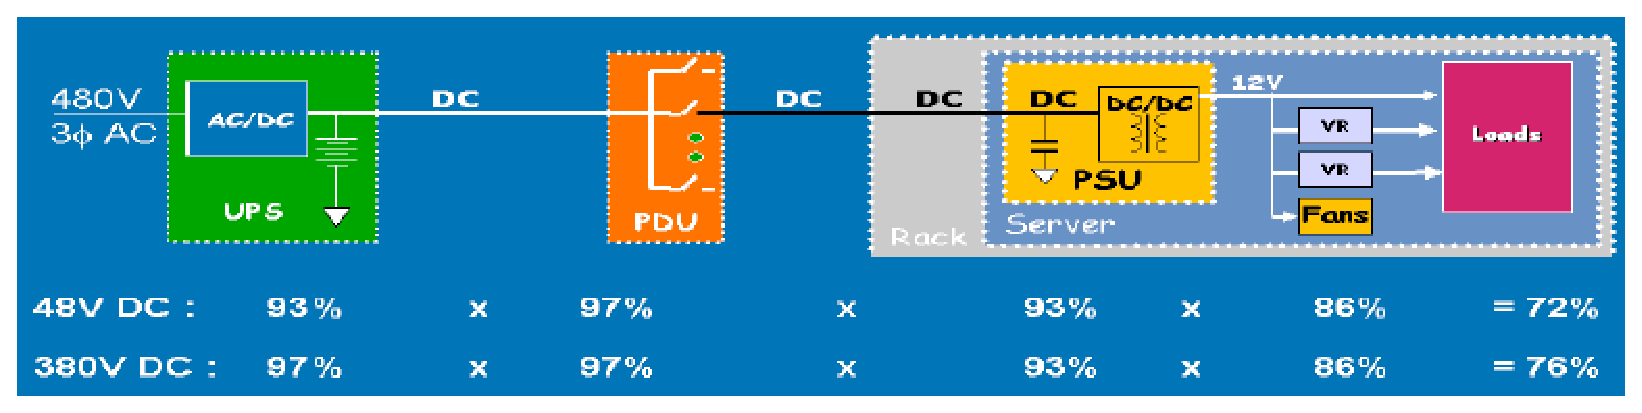
\includegraphics{graphics/facility_level_dc_efficiency}}
                    \caption{Facility-level DC architecture efficiency}
                    \label{fig:facility_level_dc_efficiency}
                \end{figure}
                In this configuration (Figure~\ref{fig:facility_level_dc_efficiency}), the DC-AC conversion in the UPS and the AC-DC conversion in the power supply are removed. It can be noted that the 480VAC-380VDC conversion in the UPS is more efficient than the 480VAC-48VDC conversion.
            
        \subsection{Data Center Infrastructure} \label{sec2:data_center_infrastructure}
            \subsubsection*{Water Cooling}
                The reasonable limit of rack power and cooling capacity for a conventional forced-air (HVAC) cooled data center is 8 kW per rack. For power densities approaching 15 kW per rack, the layout of the computing rooms and cooling facilities must be determined using specialized software (such as HP Static Smart Cooling). For racks requiring more than 15 kW, the latest cooling techniques use water (Figure~\ref{fig:power_consumption_number_servers_rack}) \cite{HPCooling07}.
                \begin{figure}[h!tb]
                    \centering
                    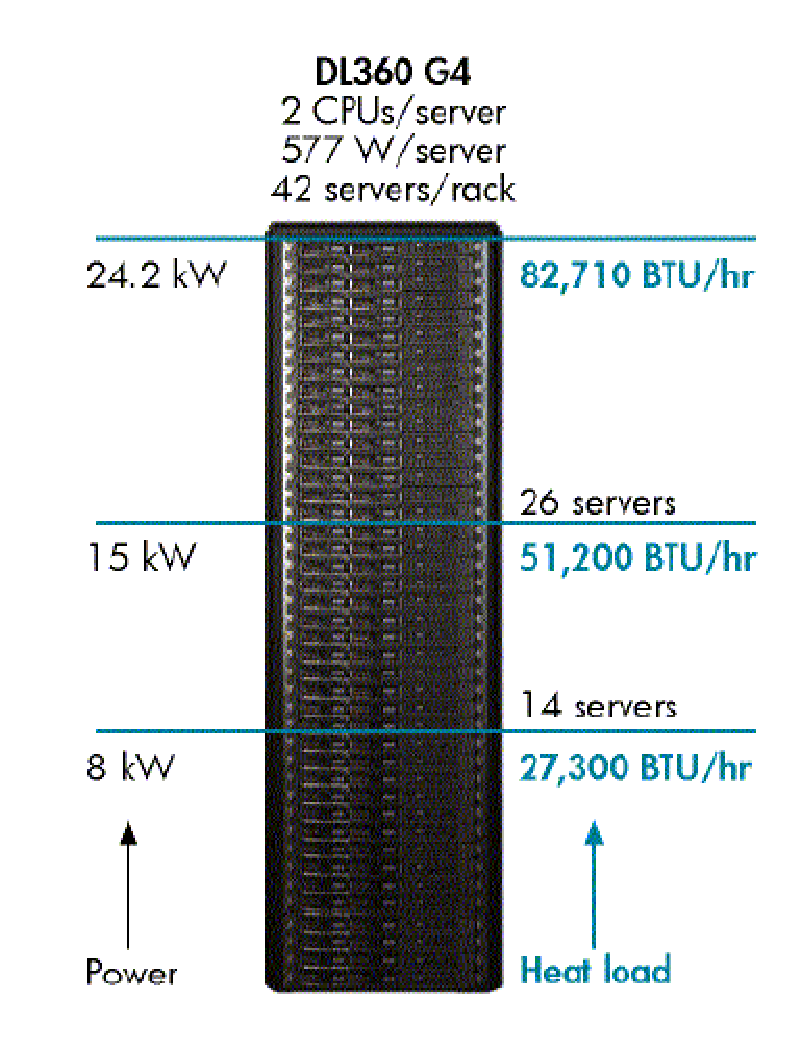
\includegraphics[scale=0.5]{graphics/power_consumption_number_servers_rack}
                    \caption{Power Consumption per Number of Servers in the Rack}
                    \label{fig:power_consumption_number_servers_rack}
                \end{figure}
                As shown in the following figure, the use of water cooling reduces in 50\% the equipment footprint, allowing greater server density. A 35 kW heat load dispersed among 4 racks could be concentrated in one single rack.
                \begin{figure}[h!tb]
                    \centering
                    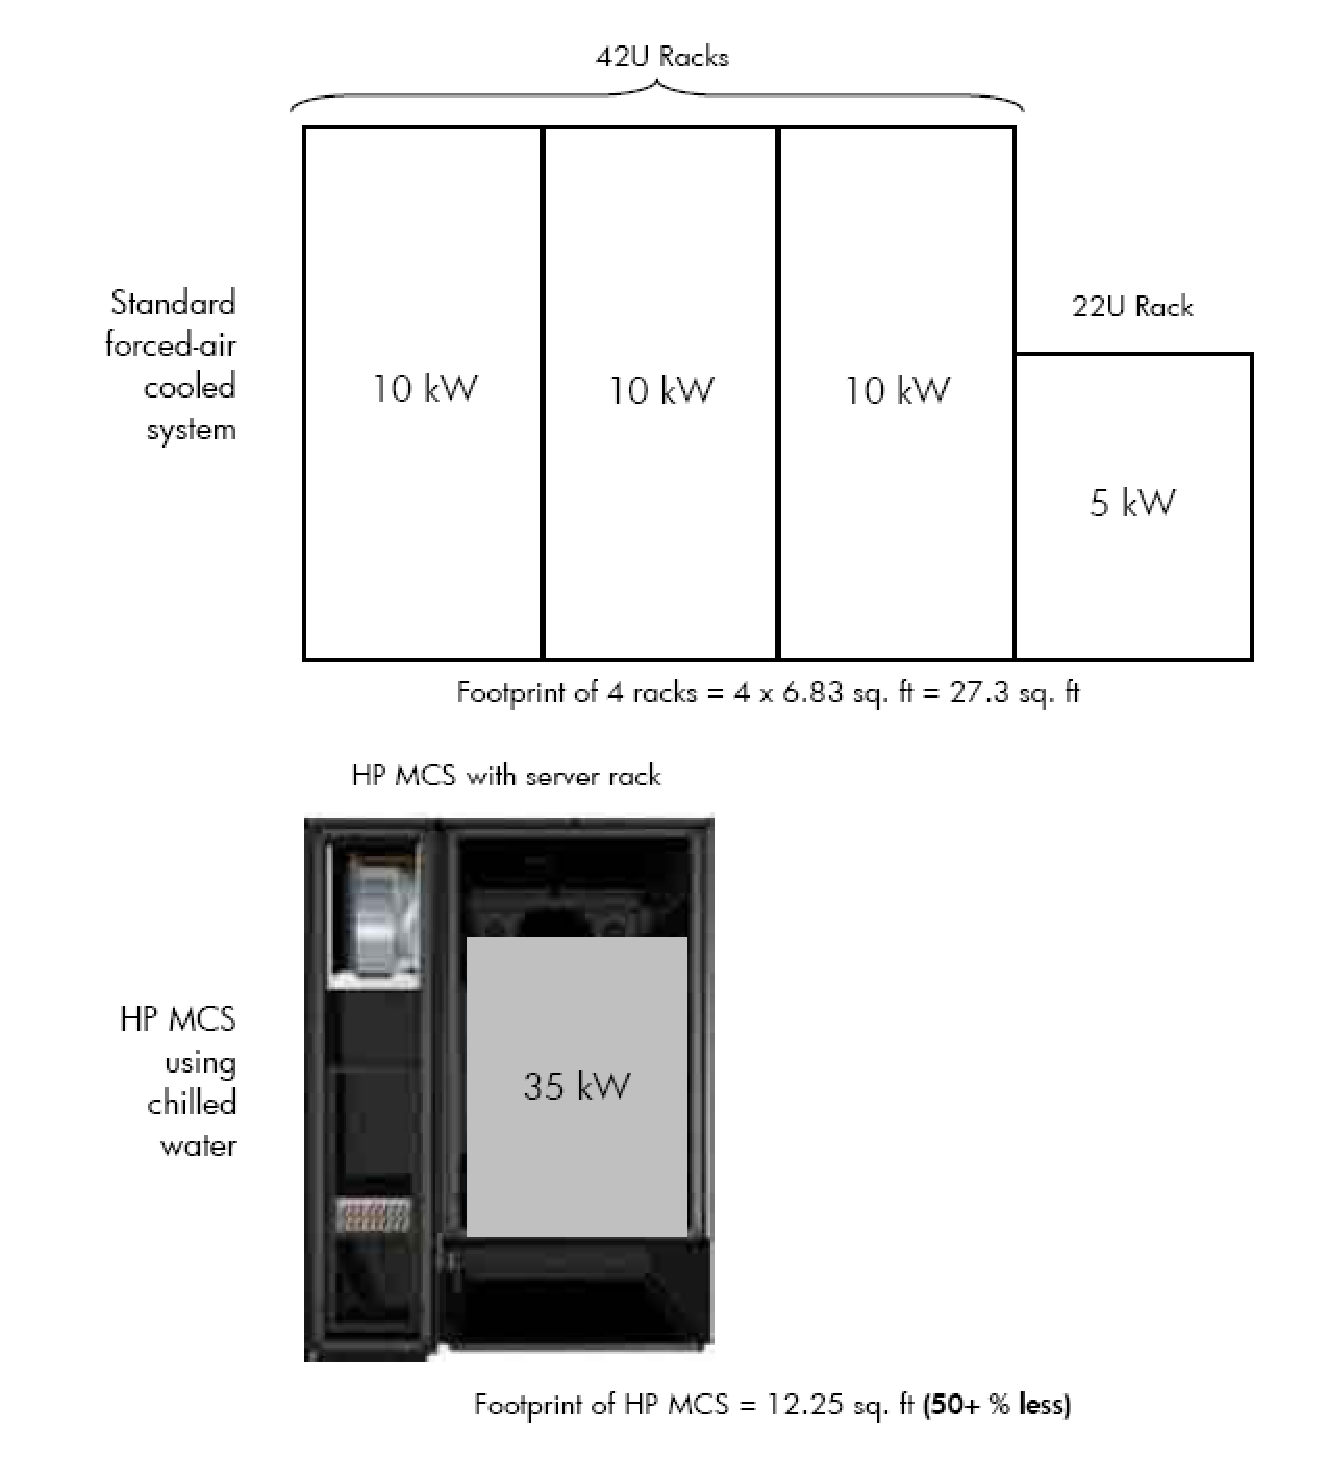
\includegraphics[scale=0.5]{graphics/footprint_reduction_for_35_heat_load}
                    \caption{Footprint Reduction for a 35 kW Heat Load}
                    \label{fig:footprint_reduction_for_35_heat_load}
                \end{figure}
                With relation to maintenance costs,
                \begin{figure}[h!tb]
                    \centering
                    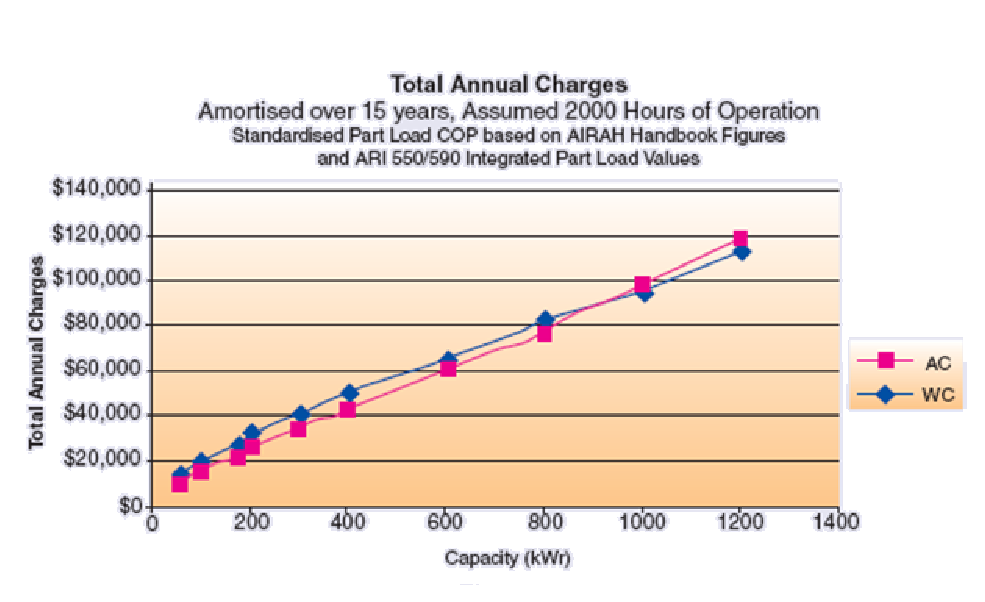
\includegraphics[scale=0.8]{graphics/economic_crossover_annualized}
                    \caption{Economic Cross-over of Annualized Charges Air-cooled to Water-cooled for 2000 Hours of Operations (in US \$)}
                    \label{fig:economic_crossover_annualized}
                \end{figure}
                \begin{figure}[h!tb]
                    \centering
                    \resizebox{\textwidth}{!}{ % Fazendo a tabela caber no espaco da pagina
                    \includegraphics[scale=0.5]{graphics/life_cycle_costs_water_cooled_air_cooled}}
                    \captionof{table}{Life Cycle Costs of Water-cooled and Air-cooled Solutions}
                    \label{tab:life_cycle_costs_water_cooled_air_cooled}
                \end{figure}
                the annual cost for water cooling and air cooling (including charges, maintenance, equipment) do not differ by a large amount as seen in  Table \ref{tab:life_cycle_costs_water_cooled_air_cooled} and Figure \ref{fig:economic_crossover_annualized}. In this way, the main benefit brought by water cooling is the footprint reduction which can increase the server density in a data center.


%%%%%%%%%%%%%%%%%%%%%%%%%%%%%%%%%%%%%
%% Master Thesis - Computer Engineering
%% Copyright 2009 Ricardo Alexandre Fiorelli, Erick Poletto
%% This document is distributed by the terms of the license
%% included in the file LICENCE.
%%%%%%%%%%%%%%%%%%%%%%%%%%%%%%%%%%%%%

%%%%%%%%%%%%%%%%%%%%%%%%%%%%%%%%%%%%%
%% Third Chapter
%% Methodology
%%%%%%%%%%%%%%%%%%%%%%%%%%%%%%%%%%%%%

\chapter{Methodology} \label{chap3:methodology}

%%%%%%%%%%%%%%%%%%%%%%%%%%%%%%%%
% Que porra � essa de Targa??? %
%%%%%%%%%%%%%%%%%%%%%%%%%%%%%%%%
\section{Dati Targa????} \label{sec3:}

\section{SiSoft SANDRA} \label{sec3:sandra}

\section{Other Tools} \label{sec3:other_tools}

\subsection{Tool1} \label{}
\subsection{Tool2} \label{}
\subsection{Tool3} \label{}

\section{Measument Methodology} \label{sec3:measurement_methodology}


%%%%%%%%%%%%%%%%%%%%%%%%%%%%%%%%%%%%%
%% Master Thesis - Computer Engineering
%% Copyright 2009 Ricardo Alexandre Fiorelli, Erick Poletto
%% This document is distributed by the terms of the license
%% included in the file LICENCE.
%%%%%%%%%%%%%%%%%%%%%%%%%%%%%%%%%%%%%

%%%%%%%%%%%%%%%%%%%%%%%%%%%%%%%%%%%%%
%% Fourth Chapter
%% Analysis and Results
%%%%%%%%%%%%%%%%%%%%%%%%%%%%%%%%%%%%%

\chapter{Analysis and Results} \label{chap4:analysis_results}
%TODO explicar o que é este capitulo, pra que ele serve, realmente PROCURAR na internet o que geralmente se coloca num capitulo assim
%TODO estudar e escrever o que aprendeu
%
    The objective of this chapter is to describe the designed component database and evaluate it against measured data and data obtained from the component manufacturers. This evaluation will determine the adequacy of power consumption data provided by the database as a means to estimate the power consumption of different machine configurations.
\section{Analysis} \label{sec4:analysis}
%TODO here it is explained the database, how it was built, the database schema and etc\ldots
%TODO
\subsection{Component Database} \label{sec4:component_database}
    The component database will be described in terms of its relations. For each relation it's semantic meaning will be explained along with the data it contains and the source of this data. The database schema is present in Figure~\ref{fig:database_schema}.

    \begin{figure}[h!tb]
        \centering
        \includegraphics[scale=0.6]{graphics/database_schema}
        \caption{Component database schema}
        \label{fig:database_schema}
    \end{figure}

    \subsubsection*{Classification relations}
        In order to provide an efficient classification of the components, four category relations were used, namely 1CAT, 2CAT, 3CAT and DEVICE. In this hierarchical disposition each component is classified in three levels by the relations 1CAT, 2CAT and 3CAT and then uniquely identified by the DEVICE relation. This classification follows the one present in the website analysed by the crawler\footnote{http://www.sisoftware.net/}.

        \paragraph*{Relation 1CAT}
            The first level of classification is very general as it just states the final usage of the component. As the components used in the database are computer components they will be defined as such in this first level.

        \paragraph*{Relation 2CAT}
            This relation fits the component into one of the main devices of a computer architecture. These are the following: processors, main memory, mass storage device, networking devices, CD/DVD player, mainboard, etc.

        \paragraph*{Relation 3CAT}
            The component is classified in a last level to provide contextual information about its usage. Processors, for example, are defined either as boxed or directly available in an OEM computer configuration. Memory can be used for servers, workstations or notebooks. Network devices can be LAN cards or networking equipment such as routers. Finally, mass storage devices are separated by technology, which can be hard-disk or flash-based.

        \paragraph*{Relation DEVICE}
            The last level is the identification of each component by an unique MPN number. This is the central relation in the database as the pricing, benchmark and characteristic relations are associated to specific components. The MPN information stored here was obtained with the use of the WEBSPHINX crawler over the SiSoftware shopping site\footnote{http://www.sisoftware.net/}. This device relation uses MPN as its key and associates for each component the 3 previous classifications, the component model/name and the date in which it was inserted in the database.
            
    \subsubsection*{Characteristic relations}
        This set of relations associate with each component its specifications, provided by the manufacturer. As SiSoftware Sandra provides these, it was be preferred source for this kind of data. Other sources such as CPU-Z reports and component datasheets were used in case the information could not be found in Sandra.
        
        \paragraph*{Relation DEVICE_CHARACTERISTIC}
            This determines the value of the characteristic being described. The value in char_value can be for example number of cores or clock frequency for a processor, disk rotation or average bandwidth for a hard drive or size and bandwidth for main memory. The attribute CHAR_ID is linked to the following relation in order to define the type of the characteristic.
            
        \paragraph*{Relation CHARACTERISTIC}
            Each characteristic, other than a value associated in the previous relation, should be described in terms of type and measurement unit. One example may be the clock frequency which is measured in MHz. In this relation the attribute CHAR_NAME would be ``clock frequency'', the attribute CHAR_UM would be ``MHz'' and the DESCRIPTION attribute would explain the meaning of the characteristic.
            
        \paragraph*{Relation SOURCE}
            For each component, the source of their characteristics could be either SiSoftware Sandra, the Web or other softwares such as CPU-Z.
                        
\subsection{Overview} \label{sec4:analysis_overview}
    % explicar que a gente pegou as coisas e separou por tabelas, tentar nao ser redundate com o que teve no cap3

\section{Results} \label{sec4:results}
%TODO falar que aqui a gente vai explicar os resultados de todos os métodos
%TODO 
\subsection{Benchmark Results} \label{sec4:benchmark_results}


%\include{chap5}

%\include{conclusao}
%%%%%%%%%%%%%%%%%%%%%%%%%%%%%%%%%%%%%
%% Master Thesis - Computer Engineering
%% Copyright 2009 Ricardo Alexandre Fiorelli, Erick Poletto
%% This document is distributed by the terms of the license
%% included in the file LICENCE.
%%%%%%%%%%%%%%%%%%%%%%%%%%%%%%%%%%%%%

%%%%%%%%%%%%%%%%%%%%%%%%%%%%%%%%%%%%%
%% Conclusions
%%%%%%%%%%%%%%%%%%%%%%%%%%%%%%%%%%%%%

\chapter*{Conclusions}

%% riassunto problema/strategia soluzione
%% risultati significativi

\section*{Perspectives and Future Developments}
% TODO
Suggestions for future developments, there are

\begin{itemize}
	\item % TODO
	\item % TODO
	\item % TODO
	\item % TODO
	\item % TODO
\end{itemize}


%\include{bibliografia}
\include{bibliography}

%\include{anexo}
\appendix
\include{appendixA}
%%%%%%%%%%%%%%%%%%%%%%%%%%%%%%%%%%%%%
%% Master Thesis - Computer Engineering
%% Copyright 2009 Ricardo Alexandre Fiorelli, Erick Poletto
%% This document is distributed by the terms of the license
%% included in the file LICENCE.
%%%%%%%%%%%%%%%%%%%%%%%%%%%%%%%%%%%%%

%%%%%%%%%%%%%%%%%%%%%%%%%%%%%%%%%%%%%
%% Appendix B
%%%%%%%%%%%%%%%%%%%%%%%%%%%%%%%%%%%%%

\chapter{Comparison Tape Drives}\label{app:comparison_tape_drives}
    \begin{table}[h!tb]
        \centering
        \begin{tabular}{|c|c|c|}
        \hline
        {\bf SDLT \&} & {\bf Native Capacity \&} & {\bf Compressed Capacity \&} \tn
        {\bf DLT Tape Drives} & {\bf Transfer Rate} & {\bf Transfer Rate} \tnhl
        {\bf DLT-S4} & 800GB at 60MB/s & 1600GB at 320MB/s \tnhl
        {\bf SDLT 600} & 300GB at 36MB/s & 600GB at 72MB/s \tnhl
        {\bf SDLT 320} & 160GB at 16MB/s & 320GB at 32MB/s \tnhl
        {\bf SDLT 220} & 110GB at 11MB/s & 220GB at 22MB/s \tnhl
        {\bf DLT 8000} & 40GB at 6MB/s & 80GB at 12MB/s \tnhl
        {\bf DLT V4} & 160GB at 10MB/s & 320GB at 20MB/s \tnhl
        {\bf DLT1} & 40GB at 3MB/s & 80GB at 12MB/s \tnhl
        {\bf DLT-VS160} & 80GB at 8MB/s & 160GB at 16MB/s \tnhl
        {\bf DLT-VS80} & 40GB at 3MB/s & 80GB at 6MB/s \tnhl
        {\bf DLT 7000} & 35GB at 5MB/s & 70GB at 10MB/s \tnhl
        {\bf DLT 4000} & 20GB at 1.5MB/s & 40GB at 3MB/s \tnhl
        {\bf DLT 2000XT} & 15GB at 1.25MB/s & 30GB at 2.5MB/s \tnhl
        \end{tabular}
        \captionof{table}[Comparison (SDLT and DLT Tape Drives) - Capacities and Transfer Rates]{Comparison Between SDLT and DLT Tape Drives Capacities and Transfer Rates}
        \label{tab:comparison_SDLT_DLT_capacities_transfer_rates}
    \end{table}
    
    \begin{table}[h!tb]
        \centering
        \begin{tabular}{|c|c|c|c|}
        \hline
        {\bf Product} & {\bf Capacity, native} & {\bf Average file access} & {\bf Data transfer rate, } \tn

            {\bf } & {\bf  (uncompressed)} & {\bf  time (first file)} & {\bf native (uncompressed)} \tnhl
                    \multicolumn{ 4}{|c|}{{\bf T-Series}} \tnhl
        \multicolumn{ 1}{|c|}{T9840A} & \multicolumn{ 1}{|c|}{20 GB} & \multicolumn{ 1}{|c|}{8 sec} & \multicolumn{ 1}{|c|}{10 MB/sec} \tnhl
        \multicolumn{ 1}{|c|}{T9840B} & \multicolumn{ 1}{|c|}{20 GB} & \multicolumn{ 1}{|c|}{8 sec} & \multicolumn{ 1}{|c|}{19 MB/sec} \tnhl
        \multicolumn{ 1}{|c|}{T9840C} & \multicolumn{ 1}{|c|}{40 GB} & \multicolumn{ 1}{|c|}{8 sec} & \multicolumn{ 1}{|c|}{30 MB/sec} \tnhl
        \multicolumn{ 1}{|c|}{T9940A} & \multicolumn{ 1}{|c|}{60 GB} & \multicolumn{ 1}{|c|}{41 sec} & \multicolumn{ 1}{|c|}{10 MB/sec} \tnhl
        \multicolumn{ 1}{|c|}{T9940B} & \multicolumn{ 1}{|c|}{200 GB} & \multicolumn{ 1}{|c|}{41 sec} & \multicolumn{ 1}{|c|}{30 MB/sec} \tnhl
                 \multicolumn{ 4}{|c|}{{\bf LTO Ultrium}} \tnhl
        \multicolumn{ 1}{|c|}{LTO Gen 1} & \multicolumn{ 1}{|c|}{100 GB} & \multicolumn{ 1}{|c|}{86-96 sec} & \multicolumn{ 1}{|c|}{15-16 MB/sec} \tnhl
        \multicolumn{ 1}{|c|}{LTO Gen 2} & \multicolumn{ 1}{|c|}{200 GB} & \multicolumn{ 1}{|c|}{64-75 sec} & \multicolumn{ 1}{|c|}{32-35 MB/sec} \tnhl
        \multicolumn{ 1}{|c|}{LTO Gen 3} & \multicolumn{ 1}{|c|}{400 GB} & \multicolumn{ 1}{|c|}{72 sec} & \multicolumn{ 1}{|c|}{80 MB/sec} \tnhl
                        \multicolumn{ 4}{|c|}{{\bf SDLT}} \tnhl
        \multicolumn{ 1}{|c|}{SDLT 320} & \multicolumn{ 1}{|c|}{160 GB} & \multicolumn{ 1}{|c|}{82 sec} & \multicolumn{ 1}{|c|}{16 MB/sec} \tnhl
        \multicolumn{ 1}{|c|}{SDLT 600} & \multicolumn{ 1}{|c|}{300 GB} & \multicolumn{ 1}{|c|}{79 sec} & \multicolumn{ 1}{|c|}{36 MB/sec} \tnhl
        \end{tabular}  
        \captionof{table}{Access times for several tape drives}
        \label{tab:access_times_tape_drives}
    \end{table}
    
    \begin{table}[h!tb]
        \centering
        \begin{tabular}{|c|c|c|} \hline
                                    &                           & {\bf Compressed}      \tn
        {\bf SDLT \&}               & {\bf Native Capacity \&}  & {\bf Capacity \&}     \tn
        {\bf DLT Tape Drives}       & {\bf Transfer Rate}       & {\bf Transfer Rate}   \tnhl
        {\bf LTO-4}                 & 800GB at 120MB/s          & 1.6TB at 240MB/s      \tn
                                    & (864GB per hour)          &                       \tnhl
        {\bf HP Ultrium 1760}       & 800GB                     & 1.6TB at 576GB/hr     \tnhl
        {\bf HP Ultrium 1840}       & 800GB at 120MB/s          & 1.6TB at 240MB/s      \tnhl
        {\bf HP Ultrium 960}        & 400GB at 80MB/s           & 800GB at 160MB/s      \tnhl
        {\bf HP Ultrium 460}        & 200GB at 30MB/s           & 400GB at 60MB/s       \tnhl
        {\bf HP Ultrium 230}        & 100GB at 15MB/s           & 200GB at 30MB/s       \tnhl
        {\bf IBM LTO-4}             & 800GB at 120MB/s          & 1.6TB at 240MB/s      \tnhl
        {\bf IBM LTO-3}             & 400GB at 80MB/s           & 800GB at 160MB/s      \tnhl
        {\bf IBM LTO-2}             & 200GB at 35MB/s           & 400GB at 70MB/s       \tnhl
        {\bf IBM LTO-1}             & 100GB at 15MB/s           & 200GB at 30MB/s       \tnhl
        {\bf Quantum LTO3}          & 400GB at 245GB/hr         & 800GB at 490GB/hr     \tnhl
        {\bf Quantum LTO3 HH}       & 400GB at 68MB/s           & 800GB at 90MB/s       \tnhl
        {\bf Quantum LTO2}          & 200GB at 123GB/hr         & 400GB at 245GB/hr     \tnhl
        {\bf Quantum LTO2HH}        & 200GB at 94GB/hr          & 400GB at 144GB/hr     \tnhl
        {\bf Tandberg Data LTO4 FH} & 800GB at 120MB/s          & 1.6TB at 240MB/s      \tnhl
        {\bf Tandberg Data LTO3 FH} & 400GB at 80MB/s           & 800GB at 160MB/s      \tnhl
        {\bf Tandberg Data LTO3 HH} & 400GB at 60MB/s           & 800GB at 120MB/s      \tnhl
        {\bf Tandberg Data LTO2 HH} & 200GB at 24MB/s           & 400GB at 48MB/s       \tnhl
        {\bf Tandberg Data LTO1 HH} & 100GB at 16MB/s           & 200GB at 32MB/s       \tnhl
        {\bf Certance LTO-1} & 100GB at 960MB/min               & 200GB at 1920MB/min   \tnhl
        \end{tabular}  
        \captionof{table}{Comparison Between LTO Tape Drives Capacities and Transfer Rates}
        \label{tab:comparison_LTO_capacities_transfer_rates}
    \end{table}
    
    

%%%%%%%%%%%%%%%%%%%%%%%%%%%%%%%%%%%%%
%% Master Thesis - Computer Engineering
%% Copyright 2009 Ricardo Alexandre Fiorelli, Erick Poletto
%% This document is distributed by the terms of the license
%% included in the file LICENCE.
%%%%%%%%%%%%%%%%%%%%%%%%%%%%%%%%%%%%%

%%%%%%%%%%%%%%%%%%%%%%%%%%%%%%%%%%%%%
%% Appendix C
%%%%%%%%%%%%%%%%%%%%%%%%%%%%%%%%%%%%%

\chapter{List of Other Energy Management Tools} \label{app:list_other_energy_management_tools}
    \section{Power To Change} \label{app:power_to_change}
    Power To Change is a widget for desktops that measures how much energy was saved when the computer is turned-off. With this application installed, when the machine is turned on, the user can receive information about how much energy and carbon footprint it was saved while it was turned off, and also, compare with global results and others.
    The widget can be downloaded from \url{http://www.hp.com/powertochange}.

    \section{PlateSpin - Recon} \label{app:power_recon}
    This software did not compose the ones used for doing this thesis. Yet, it is important to notice this, because it is almost the same of Sandra, but it provides a more incisive work on Data Centers in general. It provides workload profiling, analysis and planning of complex server consolidation, disaster recovery, capacity planning, asset management and green data center initiatives. It also provides forecasting for optimizing the data center by collecting hardware, software and services inventory for all server workloads. Furthermore, it results an statistics work for the server workloads running on data center and how their resources are being used.
    
    \section{APC Virtualization Energy Cost Calculation}\label{app:apc_virtualization_energy_cost_calculation}
        %TODO EXPLAIN about it
        \url{http://www.techworld.com/green-it/news/index.cfm?RSS&NewsID=116650}
        
        

%%%%%%%%%%%%%%%%%%%%%%%%%%%%%%%%%%%%%
%% Master Thesis - Computer Engineering
%% Copyright 2009 Ricardo Alexandre Fiorelli, Erick Poletto
%% This document is distributed by the terms of the license
%% included in the file LICENCE.
%%%%%%%%%%%%%%%%%%%%%%%%%%%%%%%%%%%%%

%%%%%%%%%%%%%%%%%%%%%%%%%%%%%%%%%%%%%
%% Appendix D
%%%%%%%%%%%%%%%%%%%%%%%%%%%%%%%%%%%%%

\chapter{Database of Components} \label{app:database_components}
    \section{SANDRA Benchmark Table Schema}\label{app:sandra_benchmark_table_schema}
        This section describes the extracted tables from SANDRA's database. They were linked through a combination of other tables from the same database in order to have more relevant data.

        \subsection*{CPU Benchmarks}\label{app:cpu_benchmarks}
            Tables~\ref{tab:CPUDataByEnergyComsumption}, \ref{tab:CPUDataByModel}, \ref{tab:CPUDataByStep}, \ref{tab:CPURefAADhryResults}, \ref{tab:CPURefAAWhetResults}, \ref{tab:CPURefMMDoubleResults}, \ref{tab:CPURefMMFloatResults}, \ref{tab:CPURefMMIntResults}, \ref{tab:RefCpuAA}, \ref{tab:RefCpuCrypt}, \ref{tab:RefCpuMM} and \ref{tab:RefCpuPwrALU} are related to benchmarks for the processor.
        % tabelas do ricardo
        \begin{table}[htbp]
        \centering
        \begin{tabular}{|l|l|l|}
        \hline
        \textbf{Field Name} & \textbf{Data Type} & \textbf{Description} \tnhl
        \textbf{ManID} & Number & Sandra manufacturer ID \tnhl
        \textbf{ClassID} & Number & Sandra CPU class ID \tnhl
        \textbf{TypeID} & Number & Sandra CPU type ID \tnhl
        \textbf{ModelID} & Number & CPUID model ID \tnhl
        \textbf{Processor Name} & Number & Name of CPU of this model \tnhl
        \textbf{RatedSpeed (MHz)} & Number & rated Speed for wattage \tnhl
        \textbf{RatedVoltage (V)} & Number & rated Vcore for wattage \tnhl
        \textbf{RatedPower (W)} & Number & rated wattage \tnhl
        \textbf{MaxTemp} & Number & in $^o$C \tnhl
        \textbf{CoolerRating} & Number & target cooler $^o$C/W rating \tnhl
        \end{tabular}
        \caption[Energy Consumption of CPU]{CPU and the energy in wattage consumed}
        \label{tab:CPUDataByEnergyComsumption}
        \end{table}
        %
        \begin{table}[htbp]
        \centering
        \begin{tabular}{|l|l|l|}
        \hline
        \textbf{Field Name} & \textbf{Data Type} & \textbf{Description} \tnhl
        \textbf{ManID} & Number & Sandra manufacturer ID \tnhl
        \textbf{ClassID} & Number & Sandra CPU class ID \tnhl
        \textbf{TypeID} & Number & Sandra CPU type ID \tnhl
        \textbf{ModelID} & Number & CPUID model ID \tnhl
        \textbf{Upgrade} & Number & Type (od, mobile, etc.) \tnhl
        \textbf{BrandID} & Number & CPUID brand ID \tnhl
        \textbf{Name} & Text & Name of CPU of this model \tnhl
        \end{tabular}
        \caption{Characteristics of the CPU organized by the Model}
        \label{tab:CPUDataByModel}
        \end{table}
        %
        \begin{table}[htbp]
        \centering
        \begin{tabularx}{\textwidth}{|>{\bfseries}l|l|X|}
        \hline
        Field Name & \textbf{Data Type} & \textbf{Description} \tnhl
        ManID & Number & Sandra manufacturer ID \tnhl
        ClassID & Number & Sandra CPU class ID \tnhl
        TypeID & Number & Sandra CPU type ID \tnhl
        ModelID & Number & CPUID model ID \tnhl
        SteppingID & Number & CPUID stepping ID (it identifies how much the design of a microprocessor has advanced from the original design) \tnhl
        Upgrade & Number & type (od, mobile, etc.) \tnhl
        BrandID & Number & CPUID brand ID \tnhl
        Steping Mask & Text & stepping mask \tnhl
        RatedSpeed (MHz) & Number & rated Speed for wattage \tnhl
        RatedVoltage (V) & Number & rated Vcore for wattage \tnhl
        RatedPower (W) & Number & rated wattage \tnhl
        MaxTemp & Number & in $^o$C \tnhl
        CoolerRating & Number & target cooler $^o$C/W rating \tnhl
        \end{tabularx}
        \caption{CPU's chatacteristcs organized by Stepping}
        \label{tab:CPUDataByStep}
        \end{table}
        %
        \begin{table}[htbp]
        \centering
        \begin{tabularx}{\textwidth}{|>{\bfseries}l|l|X|}
        \hline
        Field Name & \textbf{Data Type} & \textbf{Description} \tnhl
        CPU Type Description & Text & Processor Name \tnhl
        Os Type & Text & Architecture type (x86 or x64) \tnhl
        Speed (MHz) & Number & Frequency in MHz \tnhl
        N$^o$ Core & Number & N$^o$ of Core \tnhl
        Dhrystone Type & Text & Type of Dhrystone \tnhl
        ALU Performance & Number & Dhrystone int ALU (Arithmetic Logic Unit) value (MIPS) \tnhl
        Comment & Text & Type of Benchmark used. \tnhl
        \end{tabularx}
        \caption[Benchmarks with Dhrystone - ALU]{References to the benchmarks with Dhrystone (Arithmetic Logic Unit) performed with the processors}
        \label{tab:CPURefAADhryResults}
        \end{table}
        %
        \begin{table}[htbp]
        \centering
        \begin{tabularx}{\textwidth}{|>{\bfseries}l|l|X|}
        \hline
        Field Name & \textbf{Data Type} & \textbf{Description} \tnhl
        CPU Name & Text & Processor Name \tnhl
        Os Type & Text & Architecture type (x86 or x64) \tnhl
        Speed & Number & Frequency in MHz \tnhl
        N$^o$ Core & Number & N$^o$ Core \tnhl
        Whetstone Type & Text & Whetstone Type \tnhl
        FPU  & Number & Whetstone float FPU (Floating Point Unit) value (MFLOPS) \tnhl
        Comment & Text & Type of Benchmark used. \tnhl
        \end{tabularx}
        \caption[Benchmarks with Whetstone - FPU]{References to the benchmarks with Whetstone (Floating Point Unit) performed with the processors}
        \label{tab:CPURefAAWhetResults}
        \end{table}
        %
        \begin{table}[htbp]
        \centering
        \begin{tabular}{|l|l|l|}
        \hline
        \textbf{Field Name} & \textbf{Data Type} & \textbf{Description} \tnhl
        \textbf{CPU Name} & Text & Processor Name \tnhl
        \textbf{Os Type} & Text & Architecture type (x86 or x64) \tnhl
        \textbf{Speed} & Number & Frequency in MHz \tnhl
        \textbf{N$^o$ Core} & Number & N$^o$ Core \tnhl
        \textbf{Multimedia Double Type} & Text & Type of multimedia used \tnhl
        \textbf{Multimedia Instruction Set} & Number & Mm instruction set to use \tnhl
        \textbf{Comment} & Text & Comment on result \tnhl
        \end{tabular}
        \caption[Multimedia Benchmarks Double Results]{Multimedia benchmarks with the use of double}
        \label{tab:CPURefMMDoubleResults}
        \end{table}
        %
        \begin{table}[htbp]
        \centering
        \begin{tabular}{|l|l|l|}
        \hline
        \textbf{Field Name} & \textbf{Data Type} & \textbf{Description} \tnhl
        \textbf{CPU Name} & Text & Processor Name \tnhl
        \textbf{Os Type} & Text & Architecture type (x86 or x64) \tnhl
        \textbf{Speed} & Number & Frequency in MHz \tnhl
        \textbf{N$^o$ CPU} & Number & N$^o$ CPU \tnhl
        \textbf{Multimedia Float Type} & Text & Type of multimedia used \tnhl
        \textbf{Multimedia Instruction Set} & Number & Mm instruction set to use \tnhl
        \textbf{Comment} & Text & Comment on result \tnhl
        \end{tabular}
        \caption[Multimedia Benchmarks Float Results]{Multimedia benchmarks with the use of float}
        \label{tab:CPURefMMFloatResults}
        \end{table}
        %
        \begin{table}[htbp]
        \centering
        \begin{tabular}{|l|l|l|}
        \hline
        \textbf{Field Name} & \textbf{Data Type} & \textbf{Description} \tnhl
        \textbf{CPU Name} & Text & Processor Name \tnhl
        \textbf{Os Type} & Text & Architecture type (x86 or x64) \tnhl
        \textbf{Speed} & Number & Frequency in MHz \tnhl
        \textbf{N$^o$ CPU} & Number & N$^o$ CPU \tnhl
        \textbf{Multimedia Int Type} & Text & Type of multimedia used \tnhl
        \textbf{Multimedia Instruction Set} & Number & MM instruction set to use \tnhl
        \textbf{Comment} & Text & Comment on result \tnhl
        \end{tabular}
        \caption[Multimedia Benchmarks Integer Results]{Multimedia benchmarks with the use of integer}
        \label{tab:CPURefMMIntResults}
        \end{table}
        %
        \begin{table}[htbp]
        \centering
        \begin{tabular}{|l|l|l|}
        \hline
        \textbf{Field Name} & \textbf{Data Type} & \textbf{Description} \tnhl
        \textbf{ID} & AutoNumber & ID Number \tnhl
        \textbf{Type of Result} & Text & Type of Result \tnhl
        \textbf{Os Type} & Text & Architecture type (x86 or x64) \tnhl
        \textbf{Platform} & Number & Platform type \tnhl
        \textbf{Dateset} & Date & Date of benchmark \tnhl
        \textbf{CPU Name} & Text & Reference system name \tnhl
        \textbf{Speed} & Number & MHz \tnhl
        \textbf{Power} & Number & Power in 0.01W \tnhl
        \textbf{CPU Type} & Text & CPU Type \tnhl
        \textbf{N$^o$ Cores} & Number & N$^o$ Core units \tnhl
        \textbf{FSB Speed} & Number & FSB Speed in MHz \tnhl
        \textbf{MOPS} & Number & Combined value (MOPS) \tnhl
        \textbf{Dhrystone ALU} & Number & Dhrystone in ALU value (MIPS) \tnhl
        \textbf{Dhrystone Type} & Text & Type of Dhrystone \tnhl
        \textbf{Whetstone} & Number & Whetstone float FPU value (MFLOPS) \tnhl
        \textbf{Whetstone Type} & Text & Type of whetstone \tnhl
        \end{tabular}
        \caption[Benchmarks with Dhrystone and Whetstone]{Reference to the results of the benchmarks with Dhrystone and Whetstone}
        \label{tab:RefCpuAA}
        \end{table}
        %
        \begin{table}[htbp]
        \centering
        \begin{tabular}{|l|l|l|}
        \hline
        \textbf{Field Name} & \textbf{Data Type} & \textbf{Description} \tnhl
        \textbf{ID} & AutoNumber & ID Number \tnhl
        \textbf{Result Type} & Number & Type of result  \tnhl
        \textbf{Os Type} & Text & Architecture type (x86 or x64) \tnhl
        \textbf{Platform} & Number & Platform type \tnhl
        \textbf{Dateset} & Date/Time & Date of benchmark \tnhl
        \textbf{Name} & Text  & Reference system name \tnhl
        \textbf{Speed} & Number & Speed in MHz \tnhl
        \textbf{Power} & Number & Power in 0.01W \tnhl
        \textbf{CPU Type} & Number & CPU type \tnhl
        \textbf{N$^o$ Cores} & Number & N$^o$ Cores per unit \tnhl
        \textbf{FSB Speed} & Number & FSB Speed in MHZ \tnhl
        \textbf{Total} & Number & Total MB/s \tnhl
        \textbf{Crypto} & Number & Crypto MB/s \tnhl
        \textbf{Encryption} & Number & Encryption \tnhl
        \textbf{Descryption} & Number & Decryption \tnhl
        \textbf{Cryptographic Algorithm} & Number & Cryptographic Algorithm \tnhl
        \textbf{Cryptographic Instruction set} & Number & Cryptographic Instruction set \tnhl
        \textbf{Hash } & Number & Hash  \tnhl
        \textbf{Hash algorithm} & Number & Hash algorithm \tnhl
        \textbf{Hash Instruction set} & Number & Hash Instruction set \tnhl
        \end{tabular}
        \caption[Benchmark with Cryptography in CPUs]{Reference to the Results of the Benchmark with Cryptography in CPUs}
        \label{tab:RefCpuCrypt}
        \end{table}
        %
        \begin{table}[htbp]
        \centering
        \begin{tabular}{|l|l|l|}
        \hline
        \textbf{Field Name} & \textbf{Data Type} & \textbf{Description} \tnhl
        \textbf{ID} & AutoNumber & ID Number \tnhl
        \textbf{Result Type} & Number & Type of result  \tnhl
        \textbf{Os Type} & Text & Architecture type (x86 or x64) \tnhl
        \textbf{Platform} & Number & Platform type \tnhl
        \textbf{Dateset} & Date/Time & Date of benchmark \tnhl
        \textbf{Name} & Text  & Reference system name \tnhl
        \textbf{Speed} & Number & Speed in MHz \tnhl
        \textbf{Power} & Number & Power in 0.01W \tnhl
        \textbf{CPU Type} & Number & CPU type \tnhl
        \textbf{N$^o$ Cores} & Number & N$^o$ Cores per unit \tnhl
        \textbf{FSB Speed} & Number & FSB Speed in MHZ \tnhl
        \textbf{Total} & Number & Total \tnhl
        \textbf{MM Int} & Number & Integer \tnhl
        \textbf{MM Int Type} & Text & Integer Type \tnhl
        \textbf{MM Float} & Number & Float \tnhl
        \textbf{MM float Type} & Text & Float type \tnhl
        \textbf{MM double } & Number & Double  \tnhl
        \textbf{MM double type} & Text  & Double type \tnhl
        \end{tabular}
        \caption{Wrap up of the Benchmarks Performed with Multimedia}
        \label{tab:RefCpuMM}
        \end{table}
        %
        \begin{table}[htbp]
        \centering
        \begin{tabularx}{\textwidth}{|>{\bfseries}l|l|X|}
        \hline
        Field Name & \textbf{Data Type} & \textbf{Description} \tnhl
        ID & AutoNumber & ID Number \tnhl
        Result Type & Number & Type of result  \tnhl
        Os Type & Text & Architecture type (x86 or x64) \tnhl
        Platform & Number & Platform type \tnhl
        Dateset & Date/Time & Date of benchmark \tnhl
        Name & Text  & Reference system name \tnhl
        Speed & Number & Speed in MHz \tnhl
        Power & Number & Power in 0.01W \tnhl
        Workload Type & Number & Workload Type \tnhl
        N$^o$ Cores & Number & N$^o$ Cores per unit \tnhl
        FSB Speed & Number & FSB Speed in MHZ \tnhl
        Combine score & Number & Combined score in units \tnhl
        Efficiency & Number & Efficiency factor \tnhl
        Table & Number & A set of points of the curve generated by increasing the workload on the processor \tnhl
        \end{tabularx}
        \caption[Benchmark of Energy Consumption for Processor]{Benchmark for the energy consumption of processor by augmenting the workload}
        \label{tab:RefCpuPwrALU}
        \end{table}
        
        \subsection*{.NET Benchmarks}\label{app:dotnet_benchmarks}
        Tables~\ref{tab:RefDNetAA} and \ref{tab:RefDNetMM} are related to .NET benchmarking for the processor.
        % tabelas do erick
        \begin{table}[htbp]
        \centering
        \begin{tabularx}{\textwidth}{|>{\bfseries}X|l|X|}
        \hline
        Field Name & \textbf{Data Type} & \textbf{Description} \tnhl
        ID & Number & Component ID \tnhl
        OsType & Text & Architecture type (x86 or x64) \tnhl
        Platform & Text & Platform type (Desktop / Mobile / Server) \tnhl
        System Name & Text & CPU Model \tnhl
        Speed (MHz) & Number & CPU Speed \tnhl
        Power (.01W) & Number & CPU Power \tnhl
        CPU Type & Text & CPU Family \tnhl
        No of Core Units & Number & Number of CPU cores \tnhl
        FSB Speed (MHz) & Number & Bus Speed Obs: set as 0 for all records \tnhl
        Aggregate Performance (MOPS) & Number & Average between performance in dhrystone and whetstone benchmarks \tnhl
        Dhrystone int ALU value (MIPS) & Number & Dhrystone performance \tnhl
        Type of dhrystone & Text & Type of dhrystone benchmark (.NET) \tnhl
        Whetstone float FPU value (MFLOPS) & Number & Whetstone performance \tnhl
        Type of whetstone & Text & Type of whetstone benchmark (.NET) \tnhl
        \end{tabularx}
        \caption{.NET Arithmetic Benchmark on several CPUs}
        \label{tab:RefDNetAA}
        \end{table}
        %
        \begin{table}[htbp]
        \centering
        \begin{tabularx}{\textwidth}{|>{\bfseries}X|l|X|}
        \hline
        Field Name & \textbf{Data Type} & \textbf{Description} \tnhl
        ID & Number & Component ID \tnhl
        OsType & Text & Architecture type (x86 or x64) \tnhl
        Platform & Text & Platform type (Desktop / Mobile / Server) \tnhl
        System Name & Text & CPU Model \tnhl
        Speed (MHz) & Number & CPU Speed \tnhl
        Power (.01W) & Number & CPU Power \tnhl
        CPU Type & Text & CPU Family \tnhl
        No of Core Units & Number & Number of CPU cores \tnhl
        FSB Speed (MHz) & Number & Bus Speed
        Obs: set as 0 for all records \tnhl
        Aggregate Performance (kpixels/s) & Number & Average between performance in integer and float benchmarks \tnhl
        Int .NET Performance (kpixels/s) & Number & Int Performance \tnhl
        Float .NET Performance (kpixels/s) & Number & Float Performance \tnhl
        \end{tabularx}
        \caption{.NET Multi-Media Benchmark on several CPUs}
        \label{tab:RefDNetMM}
        \end{table}
        %
    
        \subsection*{Storage Benchmarks}\label{app:storage_benchmarks}
        Tables~\ref{tab:RefDVDRd}, \ref{tab:RefFileSystem}, \ref{tab:RefHDRd}, \ref{tab:RefHDWr} and \ref{tab:RefTape} are related to storage system.
        \begin{table}[htbp]
        \centering
        \begin{tabularx}{\textwidth}{|>{\bfseries}X|l|X|}
        \hline
        Field Name & \textbf{Data Type} & \textbf{Description} \tnhl
        ID & Number & Component ID \tnhl
        OsType & Text & Architecture type (x86 or x64) \tnhl
        Drive Model & Text & DVD drive model \tnhl
        Platform & Text & Platform type (Desktop / Mobile / Server) \tnhl
        Drive Speed (in X) & Number & 4x, 16x, etc \tnhl
        Power (.01W) & Number & Drive Power \tnhl
        Size of Media (in MB) & Number & Disk size \tnhl
        Combined Index (kB/s) & Number & Aggregate performance \tnhl
        Random Access Time (ms) & Number &  \tnhl
        Table: Drive index (kB/s) x Position on Media (\%) & Number & Performance for each position on media \tnhl
        \end{tabularx}
        \caption{DVD Benchmark (read)}
        \label{tab:RefDVDRd}
        \end{table}
        %
        \begin{table}[htbp]
        \centering
        \begin{tabularx}{\textwidth}{|>{\bfseries}l|l|X|}
        \hline
        \textbf{Field Name} & \textbf{Data Type} & \textbf{Description} \tnhl
        \textbf{ID} & Number & Component ID \tnhl
        \textbf{OsType} & Text & Architecture type (x86 or x64) \tnhl
        \textbf{Drive Model} & Text &  \tnhl
        \textbf{Platform} & Text & Platform type (Desktop / Mobile / Server) \tnhl
        \textbf{Drive Speed (RPM)} & Number &  \tnhl
        \textbf{Power (.01W)} & Number & Drive Power \tnhl
        \textbf{Drive Size (in MB)} & Number & Disk size \tnhl
        \textbf{Drive type} & Text & HD/Removable/Network \tnhl
        \textbf{Drive index (kB/s)} & Number & Aggregate performance for both reading and writing \tnhl
        \textbf{Random Access Time (ms)} & Number &  \tnhl
        \end{tabularx}
        \caption[Mounted File Systems Benchmark]{Mounted file systems benchmark. Aggregate performance for several types of drives (HD/Removable/Network)}
        \label{tab:RefFileSystem}
        \end{table}
        %
        \begin{table}[htbp]
        \centering
        \begin{tabularx}{\textwidth}{|>{\bfseries}X|l|X|}
        \hline
        Field Name & \textbf{Data Type} & \textbf{Description} \tnhl
        ID & Number & Component ID \tnhl
        OsType & Text & Architecture type (x86 or x64) \tnhl
        Platform & Text & Platform type (Desktop / Mobile / Server) \tnhl
        Drive Model & Text &  \tnhl
        Drive Speed (RPM) & Number & Obs.: set to 1000 for pen drives \tnhl
        Power (.01W) & Number & Drive Power \tnhl
        Drive Size (in MB) & Number & Disk size \tnhl
        Combined Index (kB/s) & Number & Aggregate Performance \tnhl
        Random Access Time (ms) & Number &  \tnhl
        Table: Drive index (kB/s) x Position on HD (\%) & Number & Performance for each position on HD \tnhl
        \end{tabularx}
        \caption{Physical Disk Benchmark (read)}
        \label{tab:RefHDRd}
        \end{table}
        %
        \begin{table}[htbp]
        \centering
        \begin{tabularx}{\textwidth}{|>{\bfseries}X|l|X|}
        \hline
        \textbf{ID} & \textbf{Number} & \textbf{Component ID} \tnhl
        OsType & Text & Architecture type (x86 or x64) \tnhl
        Platform & Text & Platform type (Desktop / Mobile / Server) \tnhl
        Drive Model & Text & \tnhl
        Drive Speed (RPM) & Number & Obs: set to 1000 for pen drives \tnhl
        Power (.01W) & Number & Drive Power \tnhl
        Drive Size (in MB) & Number & Disk size \tnhl
        Combined Index (kB/s) & Number & Aggregate Performance \tnhl
        Random Access Time (ms) & Number & \tnhl
        Table: Drive index (kB/s) x Position on HD (\%) & Number & Performance for each position on HD \tnhl
        \end{tabularx}
        \caption{Physical Disk Benchmark (write)}
        \label{tab:RefHDWr}
        \end{table}
        %
        
        \begin{table}[htbp]
        \centering
        \begin{tabularx}{\textwidth}{|>{\bfseries}l|l|X|}
        \hline
        \textbf{ID} & \textbf{Number} & \textbf{Component ID} \tnhl
        \textbf{OsType} & Text & Architecture type (x86 or x64) \tnhl
        \textbf{Platform} & Text & Platform type (Desktop / Mobile / Server) \tnhl
        \textbf{Drive name/model} & Text & \tnhl
        \textbf{Interface speed (Mbps)} & Number & \tnhl
        \textbf{Power (.01W)} & Number & \tnhl
        \textbf{Size of tape (MB)} & Number & \tnhl
        \textbf{Drive index (kB/s)} & Number &  \tnhl
        \textbf{Random access time (ms)} & Number & \tnhl
        \end{tabularx}
        \caption{Tape Drives Benchmark}
        \label{tab:RefTape}
        \end{table}
        %
        \subsection*{Java Benchmarks}\label{app:java_benchmarks}
        Tables~\ref{tab:RefJavaAA} and \ref{tab:RefJavaMM} are related to Java benchmars.
        \begin{table}[htbp]
        \centering
        \begin{tabularx}{\textwidth}{|>{\bfseries}X|l|X|}
        \hline
        \textbf{ID} & \textbf{Number} & \textbf{Component ID} \tnhl
        OsType & Text & Architecture type (x86 or x64) \tnhl
        Platform & Text & Platform type (Desktop / Mobile / Server) \tnhl
        System Name & Text & CPU Model \tnhl
        Speed (MHz) & Number & CPU Speed \tnhl
        Power (.01W) & Number & CPU Power \tnhl
        CPU Type & Text & CPU Family \tnhl
        No of Core Units & Number & Number of CPU cores \tnhl
        FSB Speed (MHz) & Number & Bus Speed Obs: set as 0 for all records \tnhl
        Aggregate Performance (MOPS) & Number & Average between performance in dhrystone and whetstone benchmarks \tnhl
        Dhrystone int ALU value (MIPS) & Number & Dhrystone performance \tnhl
        Type of dhrystone & Text & Type of dhrystone benchmark (Java) \tnhl
        Whetstone float FPU value (MFLOPS) & Number & Whetstone performance \tnhl
        Type of whetstone & Text & Type of whetstone benchmark (Java) \tnhl
        \end{tabularx}
        \caption[Java VM Arithmetic Benchmark]{Java VM Arithmetic Benchmark on several CPUs}
        \label{tab:RefJavaAA}
        \end{table}
        %
        \begin{table}[htbp]
        \centering
        \begin{tabularx}{\textwidth}{|>{\bfseries}X|l|X|}
        \hline
        \textbf{ID} & \textbf{Number} & \textbf{Component ID} \tnhl
        OsType & Text & Architecture type (x86 or x64) \tnhl
        Platform & Text & Platform type (Desktop / Mobile / Server) \tnhl
        System Name & Text & CPU Model \tnhl
        Speed (MHz) & Number & CPU Speed \tnhl
        Power (.01W) & Number & CPU Power \tnhl
        CPU Type & Text & CPU Family \tnhl
        No of Core Units & Number & Number of CPU cores \tnhl
        FSB Speed (MHz) & Number & Bus Speed 
        Obs: set as 0 for all records \tnhl
        Aggregate Performance (kpixels/s) & Number & Average between performance in integer and float benchmarks \tnhl
        Int Java Performance (kpixels/s) & Number & Int Performance \tnhl
        Float Java Performance (kpixels/s) & Number & Float Performance \tnhl
        \end{tabularx}
        \caption[Java VM Multi-Media Benchmark]{Java VM Multi-Media Benchmark on several CPUs}
        \label{tab:RefJavaMM}
        \end{table}
        %
        \subsection*{Memory Benchmarks}\label{app:memory_benchmarks}
        Tables~\ref{tab:RefMemBwAdv}, \ref{tab:RefMemBwLeg}, \ref{tab:RefMemLatLin} and \ref{tab:RefMemLatRnd} are related to memory benchmarks.
        \begin{table}[htbp]
        \centering
        \begin{tabularx}{\textwidth}{|>{\bfseries}X|l|X|}
        \hline
        \textbf{ID} & \textbf{Number} & \textbf{Component ID} \tnhl
        OsType & Text & Architecture type (x86 or x64) \tnhl
        Platform & Text & Platform type (Desktop / Mobile / Server) \tnhl
        Memory model & Text & Different configurations: Single chipsets or pairs of chipsets \tnhl
        Memory Speed (MHz) & Number & \tnhl
        Memory Power (.01W) & Number & \tnhl
        Memory Size (MB) & Number & Sum of capacities of all chipsets in the configuration \tnhl
        Cache speed (MHz) & Number & Obs: set as 0 for all records \tnhl
        Memory control speed (MHz) & Number & Obs: set as 0 for all records \tnhl
        Internal Graphics (0: no  1:yes) & Boolean & Set as 1 if it is a graphical card's internal memory \tnhl
        Aggregate memory performance (MB/s) & Number & Average between ALU and FPU bandwidths \tnhl
        ALU bandwidth & Number & Obs: not shown in Sandra \tnhl
        ALU type & Text & Obs: not shown in Sandra \tnhl
        FPU bandwidth & Number & Obs: not shown in Sandra \tnhl
        FPU type & Text & Obs.: not shown in Sandra \tnhl
        \end{tabularx}
        \caption[Memory Bandwidth Benchmark (newer components)]{Memory Bandwidth Benchmark (newer components) Obs: differences between ALU and FPU bandwidths only noticeable in older components}
        \label{tab:RefMemBwAdv}
        \end{table}
        %
        \begin{table}[htbp]
        \centering
        \begin{tabularx}{\textwidth}{|>{\bfseries}X|l|X|}
        \hline
        ID & \textbf{Number} & \textbf{Component ID} \tnhl
        OsType & Text & Architecture type (x86 or x64) \tnhl
        Platform & Text & Platform type (Desktop / Mobile / Server) \tnhl
        Memory model & Text & Different configurations: Single chipsets or pairs of chipsets \tnhl
        Memory Speed (MHz) & Number & \tnhl
        Memory Power (.01W) & Number & \tnhl
        Memory Size (MB) & Number & Sum of capacities of all chipsets in the configuration \tnhl
        Cache speed (MHz) & Number & Obs: set as 0 for all records \tnhl
        Memory control speed (MHz) & Number & Obs: set as 0 for all records \tnhl
        Internal Graphics (0: no  1:yes) & Boolean & Set as 1 if it is a graphical card's internal memory \tnhl
        Aggregate memory performance (MB/s) & Number & Average between ALU and FPU bandwidths \tnhl
        ALU bandwidth & Number & Obs: not shown in Sandra \tnhl
        ALU type & Text & Obs: not shown in Sandra \tnhl
        FPU bandwidth & Number & Obs: not shown in Sandra \tnhl
        FPU type & Text & Obs: not shown in Sandra \tnhl
        \end{tabularx}
        \caption[Memory Bandwidth Benchmark - (legacy components)]{Memory Bandwidth Benchmark (older, legacy components) Obs: differences between ALU and FPU bandwidths only noticeable in older components}
        \label{tab:RefMemBwLeg}
        \end{table}
        %
        \begin{table}[htbp]
        \centering
        \begin{tabularx}{\textwidth}{|>{\bfseries}X|l|X|}
        \hline
        ID & \textbf{Number} & \textbf{Component ID} \tnhl
        OsType & Text & Architecture type (x86 or x64) \tnhl
        Platform & Text & Platform type (Desktop / Mobile / Server) \tnhl
        Memory model & Text & Different configurations: Single chipsets or pairs of chipsets \tnhl
        Memory Speed (MHz) & Number & \tnhl
        Memory Power (.01W) & Number & \tnhl
        Memory Size (MB) & Number & Sum of capacities of all chipsets in the configuration \tnhl
        Cache speed (MHz) & Number & Obs: set as 0 for all records \tnhl
        Memory control speed (MHz) & Number & Obs: set as 0 for all records \tnhl
        Internal Graphics (0: no  1:yes) & Boolean & Set as 1 if it is a graphical card's internal memory \tnhl
        Combined index (ns) & Number & Aggregate latency result \tnhl
        Speed factor & Number & Obs: not shown in Sandra \tnhl
        Table: Memory latency (ns) x Test Range Size (bytes) & Number & Latency for chunks of data of different sizes (from 1kB to 64MB) \tnhl
        \end{tabularx}
        \caption[Memory Latency Benchmark - linear disposition]{Memory Latency Benchmark (linear disposition of data chunks)}
        \label{tab:RefMemLatLin}
        \end{table}
        %
        \begin{table}[htbp]
        \centering
        \begin{tabularx}{\textwidth}{|>{\bfseries}X|l|X|}
        \hline
        \textbf{ID} & \textbf{Number} & \textbf{Component ID} \tnhl
        OsType & Text & Architecture type (x86 or x64) \tnhl
        Platform & Text & Platform type (Desktop / Mobile / Server) \tnhl
        Memory model & Text & Different configurations: Single chipsets or pairs of chipsets \tnhl
        Memory Speed (MHz) & Number & \tnhl
        Memory Power (.01W) & Number & \tnhl
        Memory Size (MB) & Number & Sum of capacities of all chipsets in the configuration \tnhl
        Cache speed (MHz) & Number & Obs: set as 0 for all records \tnhl
        Memory control speed (MHz) & Number & Obs: set as 0 for all records \tnhl
        Internal Graphics (0: no  1:yes) & Boolean & Set as 1 if it is a graphical card's internal memory \tnhl
        Combined index (ns) & Number & Aggregate latency result \tnhl
        Speed factor & Number & Obs: not shown in Sandra \tnhl
        Table: Memory latency (ns) x Test Range Size (bytes) & Number & Latency for chunks of data of different sizes (from 1kB to 64MB) \tnhl
        \end{tabularx}
        \caption[Memory Latency Benchmark - random diposition]{Memory Latency Benchmark (data chunks randomly disposed throughout the memory)}
        \label{tab:RefMemLatRnd}
        \end{table}
        %
        \subsection*{Network Connection Benchmarks}\label{app:network_benchmarks}
        Tables~\ref{tab:RefNetwork}, \ref{tab:RefWebConnection} and \ref{tab:RefWireless} are related to Network connection benchmarks.
        \begin{table}[htbp]
        \centering
        \begin{tabularx}{\textwidth}{|>{\bfseries}X|l|X|}
        \hline
        \textbf{ID} & \textbf{Number} & \textbf{Component ID} \tnhl
        \textbf{OsType} & Text & Architecture type (x86 or x64) \tnhl
        \textbf{Platform} & Text & Platform type (Desktop / Mobile / Server) \tnhl
        \textbf{Network Adapter} & Text & Network card model \tnhl
        \textbf{Interface speed (kbps)} & Number & Divide by 1000 to obtain speed in Mbit \tnhl
        \textbf{Power (.01W)} & Number & \tnhl
        \textbf{Bandwidth (kB/s)} & Number & Measured speed \tnhl
        \textbf{Average latency (us)} & Number & \tnhl
        \end{tabularx}
        \caption[LAN Devices Benchmark]{LAN Devices Benchmark (network cards)}
        \label{tab:RefNetwork}
        \end{table}
        %
        \begin{table}[htbp]
        \centering
        \begin{tabularx}{\textwidth}{|>{\bfseries}l|l|X|}
        \hline
        \textbf{ID} & \textbf{Number} & \textbf{Component ID} \tnhl
        \textbf{OsType} & Text & Architecture type (x86 or x64) \tnhl
        \textbf{Platform} & Text & Platform type (Desktop / Mobile / Server) \tnhl
        \textbf{Type/name of connection} & Text & Router/modem model \tnhl
        \textbf{Interface speed (kbps)} & Number & Divide by 1000 to obtain speed in Mbit \tnhl
        \textbf{Power (.1W)} & Number & Obs: set as 0 for all records \tnhl
        \textbf{Bandwidth (kB/s)} & Number & Measured speed \tnhl
        \textbf{Average latency (ms)} & Number & \tnhl
        \end{tabularx}
        \caption[Internet Connection Benchmark]{Internet Connection Benchmark - modems/routers performance}
        \label{tab:RefWebConnection}
        \end{table}
        %
        \begin{table}[htbp]
        \centering
        \begin{tabularx}{\textwidth}{|>{\bfseries}l|l|X|}
        \hline
        \textbf{ID} & \textbf{Number} & \textbf{Component ID} \tnhl
        OsType & Text & Architecture type (x86 or x64) \tnhl
        Platform & Text & Platform type (Desktop / Mobile / Server) \tnhl
        Type/name of connection & Text & Router/modem model \tnhl
        Interface speed (kbps) & Number & Divide by 1000 to obtain speed in Mbit \tnhl
        Power (.01W) & Number & \tnhl
        Bandwidth (kB/s) & Number & Measured speed \tnhl
        Average latency (us) & Number & \tnhl
        \end{tabularx}
        \caption{Wireless Modems/Routers Performance}
        \label{tab:RefWireless}
        \end{table}



    \section{Measurement Tables}\label{app:measures_toolino}
    %TODO colocar as tabelas "completas" do excel aqui.
    % tabelas feitas com o toolino e sandra dos comps dos amigos
        \begin{table}[htbp]
        \centering
        \begin{tabularx}{\textwidth}{|>{\bfseries}l|>{\centering}X|>{\centering}X|>{\centering}X|>{\centering}X|}
        \hline
        \bf{Computer Model} & \bf{\emph{Idle} with monitor on (W)} & \bf{\emph{Idle} with monitor off (W)} & \bf{Estimated Monitor Power (W)} & \bf{Processor fully stressed} \tnhl
        HPdv3500el & 28.57 & 25.19 & 3.38 & 35.64 \tnhl
        HPdv6580el & 62.18 & 57.14 & 5.04 & 85.27 \tnhl
        Compaq-nx9420 & 78.89 & 74.65 & 4.24 & 79.64 \tnhl
        Acer Aspire 6935g & 38.67 & 33.76 & 4.91 & 55.39 \tnhl
        Acer Aspire 4720z & 44.57 & 39.88 & 4.69 & 67.28 \tnhl
        Acer Aspire 5930G & 44.48 & 39.56 & 4.92 & 62.83 \tnhl
        HP dv6000 & 43.65 & 39.12 & 4.53 & 58.95 \tnhl
        Toshiba & 54.80 & 46.03 & 8.77 & 65.73 \tnhl
        Fujistu AMILO Pa2548 & 60.28 & 55.40 & 4.88 & 87.40 \tnhl
        Samsung Q310 & 33.60 & 26.60 & 7.00 & 48.55 \tnhl
        Acer Aspire 5930G & 39.33 & 32.52 & 6.81 & 62.40 \tnhl
        HP Pavilion dv6000 & 34.06 & 29.38 & 4.68 & 48.20 \tnhl
        Sony Vaio SZ650N & 52.44 & 45.67 & 6.77 & 81.65 \tnhl
        HP Pavilion ze2000 & 37.48 & 31.48 & 6.00 & 58.34 \tnhl
        Sony Vaio v6nfw11e & 34.84 & 29.57 & 5.27 & 44.14 \tnhl
        Asus F3 Series & 47.63 & 38.98 & 8.65 & 50.33 \tnhl
        HP 550 & 41.31 & 33.60 & 7.71 & 48.11 \tnhl
        \end{tabularx}
        \caption{Measures made with the Energy Measurement Device}
        \label{tab:measures}
        \end{table}


        \begin{table}[htbp]
        \centering
        \begin{tabularx}{\textwidth}{|>{\bfseries}l|>{\centering}X|>{\centering}X|>{\centering}X|>{\centering}X|}
        \hline
        \bf{Computer Model} & \bf{Processor Benchmark (W)} & \bf{Cache \& Memory Benchmark$^a$ (W)} & \bf{Physical Disks Benchmark (W)} \tnhl
        HPdv3500el & 19.69 & 26.69 & N/A \tnhl
        HPdv6580el & 32.01 & 40.06 & 2.00 \tnhl
        Compaq-nx9420 & 26.93 & 36.16 & N/A \tnhl
        Acer Aspire 6935g & 28.03 & 35.03 & N/A \tnhl
        Acer Aspire 4720z & 19.78 & 34.57 & N/A \tnhl
        Acer Aspire 5930G & 25.13 & 32.13 & N/A \tnhl
        HP dv6000 & 25.00 & 34.23 & N/A \tnhl
        Toshiba & 22.50 & 31.24 & N/A \tnhl
        Fujistu AMILO Pa2548 & N/A & N/A & N/A \tnhl
        Samsung Q310 & 26.28 & 33.28 & N/A \tnhl
        Acer Aspire 5930G & 38.60 & 47.63 & N/A \tnhl
        HP Pavilion dv6000 & 12.95 & 31.84 & N/A \tnhl
        Sony Vaio SZ650N & 28.99 & 49.68 & N/A \tnhl
        HP Pavilion ze2000 & 14.62 & 17.86 & N/A \tnhl
        Sony Vaio v6nfw11e & 35.08 & 42.08 & N/A \tnhl
        Asus F3 Series & 12.44 & 28.53 & N/A \tnhl
        HP 550 & 29.63 & 44.42 & N/A \tnhl
        \end{tabularx}\linebreak
        $^a$ chipset + processor + memory\linebreak
        $N/A$ Not Returned a Valuable Result
        \caption{Measures Resulted from Benchmark with SANDRA}
        \label{tab:measures_sandra}
        \end{table}

        \begin{table}[htbp]
        \centering
        \begin{tabular}{|>{\bfseries}l|l|}
        \hline
        \bf{Computer Model} & \bf{Processor Model} \tnhl
        HPdv3500el & Intel Core Duo P8400 @ 2.26GHz \tnhl
        HPdv6580el & Intel Core Duo T7300 @ 2.00GHz \tnhl
        Compaq-nx9420 & Intel Core Duo T2400 @ 1.83 GHz \tnhl
        Acer Aspire 6935g & Intel Core Duo T6400 @ 2.00GHz  \tnhl
        Acer Aspire 4720z & Intel Core Duo T2310 @ 1.66 GHz \tnhl
        Acer Aspire 5930G & Intel Core 2  P7350 @ 2.0GHz \tnhl
        HP dv6000 & Intel Core Duo T5600 @ 1.83GHz \tnhl
        Toshiba & Intel Core Duo T2300 @ 1.66 GHz \tnhl
        Fujistu AMILO Pa2548 & AMD Turion 64 X2 TL-58 @ 1.9GHz \tnhl
        Samsung Q310 & Intel Core Duo P7350 @ 2.00GHz  \tnhl
        Acer Aspire 5930G & Intel Core Duo T9400 @ 2.53GHz \tnhl
        HP Pavilion dv6000 & Intel Core Duo T5450 @ 1.66GHz \tnhl
        Sony Vaio SZ650N & Intel Core Duo T7500 @ 2.20 GHz \tnhl
        HP Pavilion ze2000 & Intel Pentium M 1.60 GHz \tnhl
        Sony Vaio v6nfw11e & Intel Core Duo P8400 @ 2.26 GHz \tnhl
        Asus F3 Series & Intel Core Duo T7300 @ 2.00GHz \tnhl
        HP 550 & Intel Celeron 530 @ 1.73 GHz \tnhl
        \end{tabular}
        \caption{Processor Contained in each Measured Computer}
        \label{tab:computer_processor}
        \end{table}


        \begin{table}[htbp]
        \centering
        \begin{tabularx}{0.7\textwidth}{|l|>{\centering}X|}
        \hline
        \bf{Processor Model} & \bf{Processor nominal power (W)} \tnhl
        Intel Core Duo P8400 @ 2.26GHz & 25 \tnhl
        Intel Core Duo T7300 @ 2.00GHz & 35 \tnhl
        Intel Core Duo T2400 @ 1.83 GHz & 31 \tnhl
        Intel Core Duo T6400 @ 2.00GHz  & 35 \tnhl
        Intel Core Duo T2310 @ 1.66 GHz & 35 \tnhl
        Intel Core 2  P7350 @ 2.0GHz & 25 \tnhl
        Intel Core Duo T5600 @ 1.83GHz & 34 \tnhl
        Intel Core Duo T2300 @ 1.66 GHz & 31 \tnhl
        AMD Turion 64 X2 TL-58 @ 1.9GHz & 31 \tnhl
        Intel Core Duo P7350 @ 2.00GHz  & 25 \tnhl
        Intel Core Duo T9400 @ 2.53GHz & 35 \tnhl
        Intel Core Duo T5450 @ 1.66GHz & 35 \tnhl
        Intel Core Duo T7500 @ 2.20 GHz & 35 \tnhl
        Intel Pentium M 1.60 GHz & 35 \tnhl
        Intel Core Duo P8400 @ 2.26 GHz & 25 \tnhl
        Intel Core Duo T7300 @ 2.00GHz & 35 \tnhl
        Intel Celeron 530 @ 1.73 GHz & 27 \tnhl
        \end{tabularx}
        \caption{Manufacturer Specification}
        \label{tab:manufacturer_specification}
        \end{table}


    %\section{Characteristics of Measured Computers} \label{app:characteristics_measured_computers}
    %TODO


    \section{Database Schema}\label{app:database_schema}
    %TODO
        \begin{sidewaysfigure}[htbp]
            \centering
            \resizebox{\textwidth}{!}{ % Fazendo a tabela caber no espaco da pagina
            \includegraphics{graphics/database_schema}}
            \caption{Database Schema}
            \label{fig:database_schema}
        \end{sidewaysfigure}




%%%%%%%%%%%%%%%%%%%%%%%%%%%%%%%%%%%%%%
%% Master Thesis - Computer Engineering
%% Copyright 2009 Ricardo Alexandre Fiorelli, Erick Poletto
%% This document is distributed by the terms of the license
%% included in the file LICENCE.
%%%%%%%%%%%%%%%%%%%%%%%%%%%%%%%%%%%%%

%%%%%%%%%%%%%%%%%%%%%%%%%%%%%%%%%%%%%
%% Ferramentas
%%%%%%%%%%%%%%%%%%%%%%%%%%%%%%%%%%%%%

\documentclass{abnt}
%\usepackage[brazil]{babel} 
\usepackage[english]{babel}
\usepackage[latin1]{inputenc}

\begin{document}

\pretextualchapter{}

\vspace{20cm}

\begin{center}
\textbf{Produced with} \\
\textbf{\LaTeX}
\end{center}

\end{document}


\end{document}

